\documentclass[5p,times]{elsarticle}
\usepackage{amsmath,amsfonts,amssymb}
\usepackage{algorithm}
\usepackage{algorithmic}
\usepackage{placeins}
\usepackage{array}
\usepackage{subfig}
\usepackage{textcomp}
\usepackage{url}
\usepackage{graphicx}
\usepackage{booktabs}
\usepackage{makecell}
\usepackage{multirow}
\usepackage{adjustbox}
\usepackage{tabularx}
\usepackage{amsthm}

% Compact, flexible float placement for the journal's two-column layout.
\setcounter{topnumber}{4}
\setcounter{dbltopnumber}{4}
\renewcommand{\topfraction}{0.95}
\renewcommand{\dbltopfraction}{0.95}
\renewcommand{\textfraction}{0.05}
\renewcommand{\floatpagefraction}{0.85}
\renewcommand{\dblfloatpagefraction}{0.85}
\setlength{\textfloatsep}{8pt plus 2pt minus 2pt}
\setlength{\dbltextfloatsep}{8pt plus 2pt minus 2pt}
\setlength{\emergencystretch}{2em}
\urlstyle{same}

\graphicspath{{figures/}{figures_en/}}

\journal{Journal of Parallel and Distributed Computing}

\theoremstyle{plain}
\newtheorem{theorem}{Theorem}
\newtheorem{lemma}[theorem]{Lemma}
\newtheorem{proposition}[theorem]{Proposition}
\newtheorem{corollary}[theorem]{Corollary}
\newtheorem{assumption}[theorem]{Assumption}

\theoremstyle{definition}
\newtheorem{definition}[theorem]{Definition}

\theoremstyle{remark}
\newtheorem{remark}[theorem]{Remark}

\newcommand{\tabref}[1]{Table~\ref{#1}}
\newcommand{\figref}[1]{Fig.~\ref{#1}}
\newcommand{\secref}[1]{Section~\ref{#1}}
\newcommand{\equref}[1]{(\ref{#1})}

\makeatletter
\newenvironment{breakablealgorithm}
{%
	\par\addvspace{\intextsep}
	\refstepcounter{algorithm}%
	\hrule height 0.8pt depth 0pt
	\kern 2pt
	\renewcommand{\caption}[2][\relax]{%
		\noindent\textbf{\ALG@name~\thealgorithm}\ ##2\par
		\ifx\relax##1\relax
		\addcontentsline{loa}{algorithm}{\protect\numberline{\thealgorithm}##2}%
		\else
		\addcontentsline{loa}{algorithm}{\protect\numberline{\thealgorithm}##1}%
		\fi
		\kern 2pt
		\hrule height 0.8pt depth 0pt
		\kern 2pt
	}%
}
{%
	\kern 2pt
	\hrule height 0.8pt depth 0pt
	\par\addvspace{\intextsep}
}
\makeatother

\begin{document}
	
	\begin{frontmatter}
		
		\title{Dynamic Collaboration Mode Selection in Hierarchical Federated Learning}
		
		\author[bupt1,bupt2,bupt3]{Tingting Yang}
		\author[bupt1,bupt2,bupt3]{Wenbo Zhang\corref{cor1}}
		\ead{zhangwb@bupt.edu.cn}
		\cortext[cor1]{Corresponding author.}
		\author[bupt1,bupt2,bupt3]{Shaohua Liu}
		\author[bupt1,bupt2,bupt3]{Lihua Zhang}
		\author[bupt1,bupt2,bupt3]{Xinyuan Lin}
		\author[bupt1,bupt2,bupt3]{Qian Liu}
		
		\affiliation[bupt1]{
			organization={School of Mathematical Sciences, Beijing University of Posts and Telecommunications},
			city={Beijing},
			country={China}
		}
		
		\affiliation[bupt2]{
			organization={State Key Laboratory of Information Photonics and Optical Communications (Beijing University of Posts and Telecommunications)},
			city={Beijing},
			country={China}
		}
		
		\affiliation[bupt3]{
			organization={Key Laboratory of Mathematics and Information Networks (Beijing University of Posts and Telecommunications), Ministry of Education},
			city={Beijing},
			country={China}
		}
		
		\begin{abstract}
			Hierarchical federated learning enables collaboration among Cloud, Edge, and end devices, but fixed collaboration schemes may not adapt effectively to heterogeneous and changing system conditions.
			To address this challenge, a dynamic collaboration mode selection framework is proposed. Three collaboration modes are considered: Edge aggregation with asynchronous Cloud updates ($FL_E$), multistage Edge aggregation followed by Cloud aggregation ($FL_{EC}$), and direct Cloud aggregation ($FL_C$).
			To evaluate candidate mode distributions, a historical aggregate update deviation score is constructed by combining mode specific historical update deviations with the aggregation weights of the corresponding Cloud update units.
			The proposed framework combines this score with estimated system latency into a joint utility and dynamically selects feasible mode distributions under resource and lifetime privacy constraints.
			Experiments on Fashion MNIST with LeNet 5 evaluate the relationship between the proposed deviation score and subsequent learning performance. 
			Experimental results show that the rankings
			of the examined candidate distributions by
			the proposed score are consistent with their
			subsequent loss reductions, providing
			empirical support for the effectiveness
			of the proposed score.
			Further experiments demonstrate how different
			utility weights affect learning performance
			and cumulative system latency.
		\end{abstract}
		
		\begin{keyword} 
			hierarchical federated learning \sep cloud-edge-end collaboration \sep dynamic collaboration mode selection \sep differential privacy \sep device heterogeneity 
		\end{keyword}
		
	\end{frontmatter}
	\section{Introduction}
	\label{sec:introduction}
	Federated learning (FL) enables multiple end devices to collaboratively train a shared model without transferring raw data to a central server~\cite{fedavg,ZHAO2026108518}. In AIoT systems, however, participating devices differ substantially in computational capability, memory capacity, communication quality, and local data distribution. Cloud-edge-end hierarchical federated learning (HFL) introduces edge servers between end devices and the cloud, providing intermediate aggregation and computation capabilities while reducing direct communication with the cloud~\cite{hfl,FLaTEC2026,yang2026hierarchical}.
	
	Data and system heterogeneity can limit the effectiveness of fixed cloud-edge-end collaboration schemes across clients and training rounds. First, non-IID data can cause
	local updates to drift in different directions and can degrade simple weighted
	aggregation~\cite{fedavgm,fedprox,scaffold,khan2026accelerating,11214447}.
	Second, system capabilities are heterogeneous. A weak end device may be unable
	to handle the same workload or meet the same deadline as a stronger device,
	whereas an edge or cloud server can undertake more computation~\cite{wang2019adaptivefl,FAN2026108249}.
	A mode that suits one client in one round may be inefficient or infeasible
	for the same client in another round, or for another client.
	
	Existing work on HFL and cloud-edge-end collaboration has covered personalization,
	resource allocation, wireless scheduling, heterogeneous models, and split
	training~\cite{Personalizedhfl,JSJX202502007,dinh2021wirelessfl,BSBODP,mazloomi2025multiserver,SFETEC,11185336,YAO2026108495}.	
	These studies address different aspects of
	collaborative training. However, heterogeneous
	client capabilities, non IID data, and changing
	communication conditions can affect the suitability
	of different collaboration modes across training
	rounds. A fixed mode assignment may therefore
	fail to maintain a desirable balance between
	learning related update behavior and system
	latency under resource and lifetime privacy
	constraints.	
	
	To address this problem, three collaboration
	modes are considered in the proposed framework.	
	In $FL_E$, clients perform one local training
	stage and submit their updates to the Edge for
	aggregation. The resulting Edge model is
	returned to clients without waiting for Cloud
	aggregation, while the aggregated Edge update
	is asynchronously forwarded to the Cloud to
	contribute to global aggregation.
	In $FL_{EC}$, clients perform multiple local
	training and Edge aggregation stages before
	the final Edge update is forwarded to the Cloud.
	In $FL_C$, client updates are directly transmitted
	to the Cloud for aggregation.
	
	These modes provide different aggregation paths
	and training stage arrangements, making their
	suitability dependent on the current system
	conditions. A mode distribution that is suitable
	under one set of conditions may not remain
	effective as client resources, communication
	conditions, and update characteristics change.
	Therefore, the proposed method dynamically
	selects a feasible distribution of clients among
	the three modes from a finite candidate set.
	
	Each candidate is evaluated using a historical
	aggregate update deviation score and estimated
	system latency, subject to resource and lifetime
	privacy constraints. These two quantities form
	the joint utility for mode selection. The deviation
	score serves as a decision signal rather than a
	direct measure of model accuracy. The learning
	performance of the selected strategies is then
	evaluated experimentally.
	
	
	The main contributions of this paper are as follows:
	\begin{itemize}
		
		\item A dynamic collaboration mode selection
		framework is developed for hierarchical
		federated learning with three collaboration
		modes, $FL_E$, $FL_{EC}$, and $FL_C$,
		distinguished by their aggregation paths
		and training stage arrangements.
		A finite set of candidate mode distributions
		is used to represent different client
		assignments across these modes.
		
		\item A historical aggregate update deviation
		score is constructed by combining mode
		specific historical update deviations
		with the aggregation weights of the
		corresponding Cloud update units.
		The proposed score is integrated with
		estimated system latency into a normalized
		joint utility to evaluate feasible candidate
		mode distributions under resource and
		lifetime privacy constraints.
		
		\item Simulation experiments are conducted
		to evaluate the proposed framework.
		The results provide empirical support
		for the effectiveness of the proposed
		deviation score by showing consistency
		between candidate score rankings and
		subsequent loss reductions.
		Further comparisons characterize the
		tradeoffs between learning performance
		and system latency under different
		utility preferences and switching controls.
		
	\end{itemize}
	
	
	The remainder of this paper is organized as follows.
	Section~\ref{sec:related_work} reviews related studies
	on hierarchical federated learning and cloud-edge-end
	collaboration.
	Section~\ref{sec:model} introduces the system model
	and formulates the historical aggregate deviation
	contribution and system latency under resource
	and lifetime privacy constraints.
	Section~\ref{sec:algorithm} presents the proposed
	dynamic collaboration selection algorithm.
	Section~\ref{sec:experiment} evaluates its performance
	through experiments.
	Finally, Section~\ref{sec:conclusion} concludes the paper.
	
	\section{Related Work}
	\label{sec:related_work}
	Existing research on hierarchical federated
	learning covers resource optimization,
	collaborative training and aggregation,
	and privacy protection. This section
	reviews representative studies in these
	three research directions.
	\subsection{HFL Under Heterogeneous Environments}
	
	Hierarchical federated learning introduces
	intermediate Edge aggregation to improve
	communication efficiency in distributed
	training~\cite{hfl}. Resource constraints
	and differences in client capabilities have
	motivated the adaptation of training and
	communication parameters.
	PHFL employs model pruning and jointly
	adjusts pruning ratios, processor frequencies,
	and transmission power to address limited
	bandwidth and heterogeneous device
	capabilities~\cite{phfl}.
	Xu et al. investigate adaptive control of
	local update frequency and model compression
	to improve training efficiency~\cite{xu2022adaptive}.
	
	More recently, Su et al. jointly optimize
	aggregation frequencies and computation
	and communication resources in hierarchical
	federated learning~\cite{su2025adaptivehfl}.
	Wei et al. introduce a digital twin based
	framework that dynamically adjusts aggregation
	deadlines and resource allocation in hierarchical
	federated learning for IoT
	environments~\cite{wei2026dthfl}.
	
	Data heterogeneity has also motivated client
	clustering and model personalization.
	Clustered FL organizes clients into groups
	according to similarities in their training
	characteristics~\cite{sattler2020clustered}.
	Other studies investigate shared representations
	and personalized hierarchical federated learning
	to accommodate differences in local data
	distributions~\cite{collins2021exploiting,
		Personalizedhfl}.
	Together with the resource management approaches
	discussed above, these studies address
	heterogeneous federated training through
	model adaptation, aggregation control,
	and resource optimization.
	
	\subsection{Cloud-Edge-End Collaborative Federated Learning}
	
	Collaborative FL across the Cloud, Edge, and Local
	tiers can be organized through different training
	and aggregation mechanisms. FedAgg employs bridge
	samples and online knowledge distillation to
	transfer knowledge between models of different
	sizes across the three tiers~\cite{BSBODP}.
	FLaTEC distributes model components between
	devices and Edge servers and applies knowledge
	distillation to support efficient collaborative
	training~\cite{FLaTEC2026}.
	Fed3Scale introduces a collaborative framework
	that combines training and aggregation across
	the three tiers with semi supervised
	learning~\cite{fed3scale}.
	
	Aggregation synchronization has also been
	investigated to improve training efficiency.
	FedSA employs a semi asynchronous mechanism
	that aggregates a specified number of received
	client updates instead of waiting for all
	participating clients~\cite{Ma2021}.
	This approach adjusts aggregation timing to
	reduce the waiting delay associated with
	synchronous training.
	
	
	These studies illustrate different approaches to organizing collaborative training and aggregation across multiple tiers.	The diversity of aggregation paths and synchronization requirements provides a basis for dynamic collaboration mode selection in hierarchical federated learning.
	
	
	
	\subsection{Privacy Preserving HFL}
	
	Although raw training data remain on local devices,
	model updates may still reveal sensitive information
	about the training data~\cite{zhu2019dlg}.
	Differential privacy (DP) has been widely investigated
	to limit information leakage during federated
	training~\cite{dwork2006calibrating}.
	
	Privacy preservation in HFL has been studied
	through different mechanisms.
	Chen et al. investigate personalized privacy
	protection using group local DP, incorporating
	randomized response and shuffling~\cite{GLDP}.
	Xu et al. propose ADPFL, which adapts privacy
	budget allocation, gradient clipping, and
	client selection during training~\cite{xu2025adpfl}.
	Wang et al. develop a client sampling framework
	that protects both communicated model information
	and information revealed by client sampling
	decisions~\cite{11267456}.
	
	Other studies combine multiple privacy mechanisms
	within hierarchical architectures.
	Kalafatelis et al. integrate client level DP,
	secure aggregation, and homomorphic encryption
	for hierarchical learning across data
	spaces~\cite{PPHFL}.
	Islam et al. incorporate DP and personalization
	into hierarchical fog federated learning
	for IoT intrusion detection~\cite{islam2025pphffl}.
	
	These studies investigate privacy preservation
	through different mechanisms and adaptive
	privacy control strategies.
	In the proposed framework, DP-SGD is applied
	during local training, and RDP accounting
	tracks the accumulated privacy loss across
	training rounds~\cite{abadi2016deep,mironov2017renyi}.
	The lifetime privacy budget is incorporated
	into the feasibility assessment of candidate
	collaboration mode distributions, together
	with resource constraints.
	Privacy constraints are therefore considered
	alongside historical update deviation and
	estimated system latency during mode selection.
	\section{Model Construction}
	\label{sec:model}
	\subsection{Collaborative Mode and Transmission Modeling}
	\label{sec:link_model}
	We consider a three-tier federated learning system
	consisting of \(N\) clients, a set of edge servers,
	and a central cloud server. Each client \(i\) is
	associated with an edge server \(e(i)\). At round
	\(t\), the system assigns a collaboration mode
	\(h_i^t\in\mathcal H\) to each participating client,
	allowing training and aggregation to be organized
	across different tiers.
	
	\textbf{Collaboration modes.}
	Three collaboration modes are considered in the 
	cloud-edge-end architecture, which are distinguished 
	by their aggregation paths and client-side synchronization 
	requirements.
	
	In Edge based Federated Learning ($FL_E$),
	clients perform local training and submit
	their updates to the Edge for aggregation.
	After Edge aggregation, the resulting Edge
	model is returned to clients independently
	of the Cloud aggregation process. Meanwhile,
	the aggregated Edge update is asynchronously
	forwarded to the Cloud and contributes to
	global aggregation. In 
	Edge--Cloud Federated Learning ($FL_{EC}$), a group of 
	clients associated with the same Edge participates in a 
	multi-stage collaborative process. The Edge performs $E_B$ 
	processing stages before submitting a single final joint 
	update to the Cloud for global aggregation. In Cloud-based 
	Federated Learning ($FL_C$), clients directly submit their 
	locally trained updates to the Cloud for aggregation without 
	intermediate Edge aggregation.
	
	Let \(L\), \(E\), and \(C\) denote the Local, Edge,
	and Cloud tiers, respectively. The three candidate
	collaboration modes are defined as
	\begin{equation}
		\mathcal H =
		\{\mathrm{FL_E},\mathrm{FL_{EC}},\mathrm{FL_C}\}.
		\label{eq:three_modes}
	\end{equation}
	In all three modes, raw training data remain on
	the client. Local model updates or Edge-aggregated
	updates are transmitted according to the selected
	collaboration mode.
	
	
	\subsubsection{Collaborative Training Blocks and Mode Flows}
	
	Let \(L_B\) denote the number of local training
	steps in each block, and let \(T_L(L_B)\) represent
	the corresponding local training process followed
	by model update generation.
	During local training, 
	gradients computed for each example are clipped, 
	and Gaussian noise is added to the clipped gradients using differentially private stochastic gradient descent.
	Let \(A_E\) and \(A_C\)
	denote aggregation at the Edge and Cloud,
	respectively.
	For the \(FL_{EC}\) mode, \(E_B\) denotes
	the number of Edge processing and aggregation
	stages. At each stage, clients perform
	\(L_B\) local training steps using the latest
	model received from the Edge. After each
	stage, the aggregated model is returned to
	the clients for the next stage. The final
	aggregated update is denoted by
	\(\Delta_e^{(E_B)}\).
	\begin{equation}
		\begin{aligned}
			\mathrm{FL_E}:~~&
			T_L(L_B)
			\xrightarrow{\mathrm{upd}} A_E
			\xrightarrow{\mathrm{async\ upd}} A_C,\\
			\mathrm{FL_{EC}}:~~&
			T_L(L_B)
			\xrightarrow{\mathrm{upd}} \Delta_e^{(E_B)}
			\xrightarrow{\mathrm{upd}} A_C,\\
			\mathrm{FL_C}:~~&
			T_L(L_B)
			\xrightarrow{\mathrm{upd}} A_C.
		\end{aligned}
		\label{eq:mode_flows}
	\end{equation}
	Here, The arrows indicate the direction of information flow.
	The label \(\mathrm{upd}\) indicates the transmission
	of a model update to the next aggregation stage.
	The label \(\mathrm{async\ upd}\) indicates
	asynchronous update transmission without requiring
	clients to wait for Cloud-side aggregation.
	
	Figure~\ref{fig:eecblockflow} illustrates the
	execution structures of the three collaboration
	modes. Figures (a)--(c) show the execution and
	aggregation processes of \(FL_E\), \(FL_{EC}\),
	and \(FL_C\), respectively, while Fig.~(d)
	compares the three modes from the perspective
	of an individual client. Filled circles, hollow
	circles, and hollow diamonds represent the
	Local, Edge, and Cloud tiers, respectively.
	Dashed arrows indicate model update transmissions,
	and circular arrows represent aggregation
	operations. Spring-like marks indicate that the transmitted
	model updates contain noise introduced by
	client-side DP-SGD during local training.
	
	\begin{figure}[t]
		\centering
		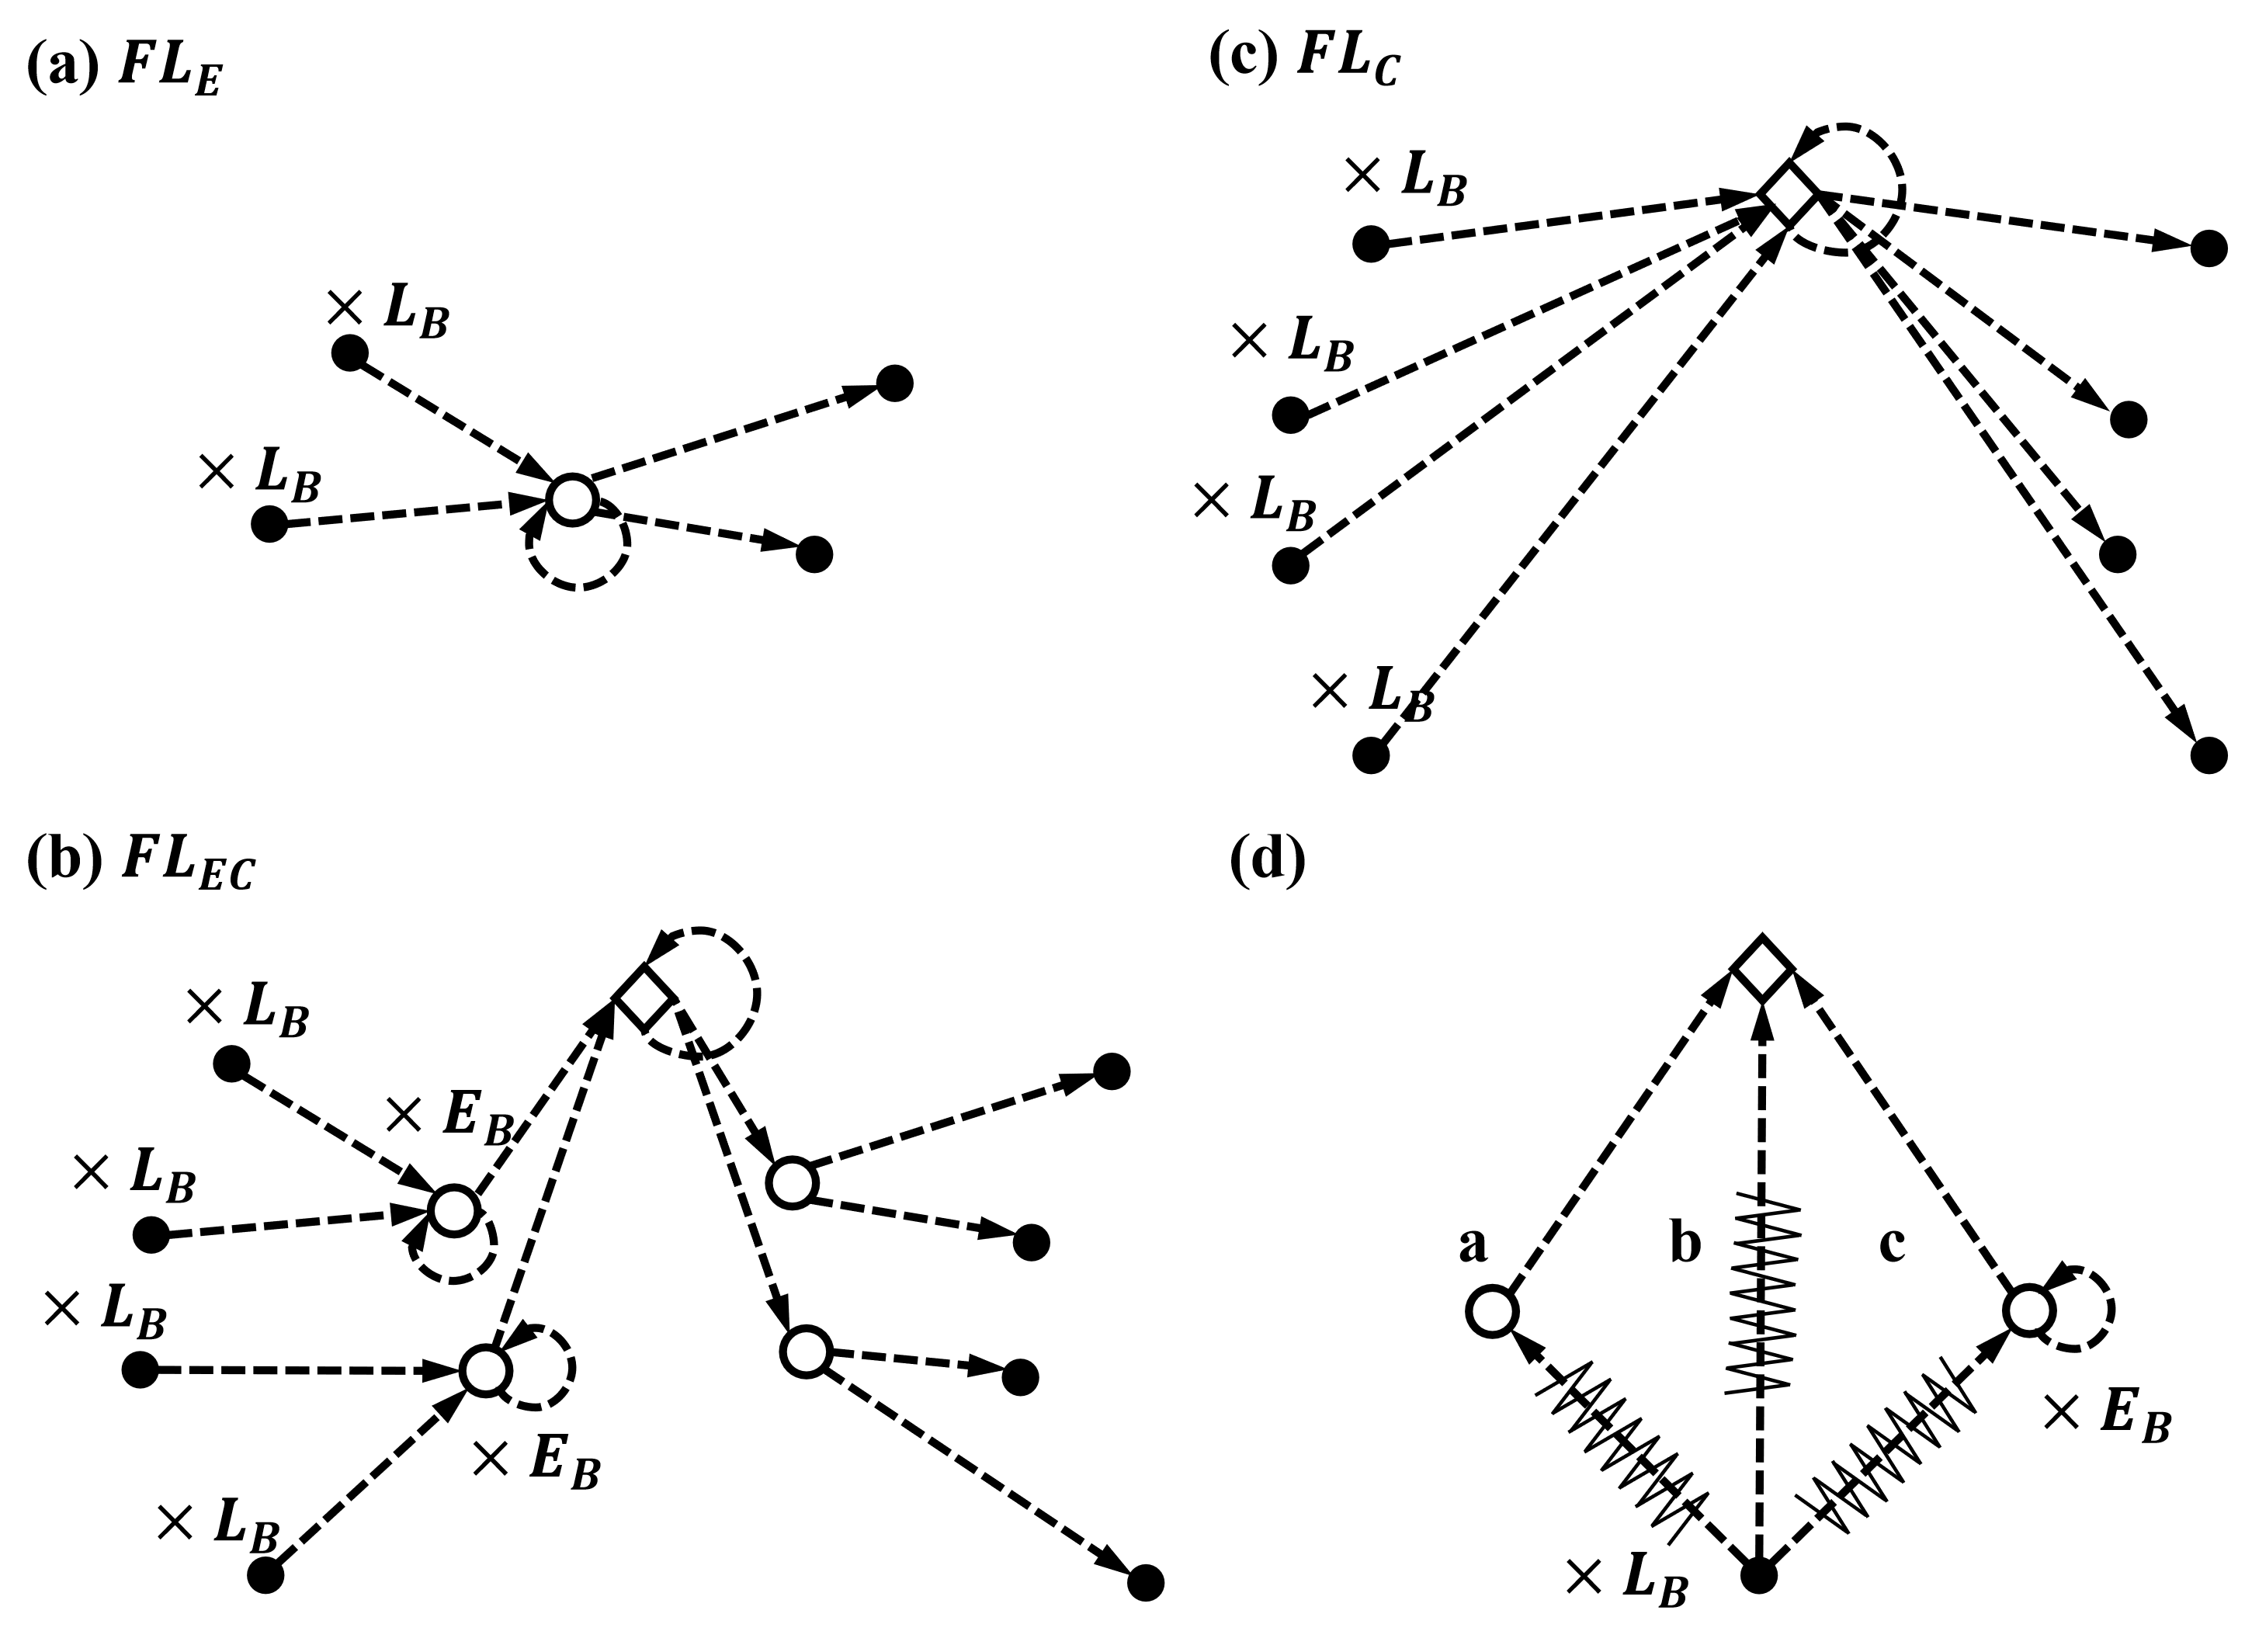
\includegraphics[width=\columnwidth]{eecblockflow.png}
		\caption{Execution structures of the three collaboration modes in the cloud-edge-end architecture.}
		\label{fig:eecblockflow}
	\end{figure}
	
	\subsection{Lifetime Privacy Accounting}
	\label{sec:privacy_model}
	
	Sample-level differential privacy~\cite{dwork2014the}
	is enforced during local training through the
	differentially private stochastic gradient descent
	mechanism~\cite{abadi2016deep}, in which gradients
	are clipped and Gaussian noise is added to the
	clipped gradients. The resulting model updates
	carry this noise when transmitted across tiers. For each client,
	R\'enyi differential privacy (RDP)~\cite{mironov2017renyi}
	is used to accumulate privacy loss across
	training rounds. Let \(\mathcal A\) denote
	the set of R\'enyi orders~\cite{vanerven2014renyi}. 
	For a Gaussian
	mechanism with noise multiplier \(\sigma\),
	the RDP cost at order \(\alpha\in\mathcal A\)
	is \(\rho(\alpha,\sigma)=\alpha/(2\sigma^2)\).
	
	Let \(m_i^t\) denote the number of Gaussian
	mechanisms applied to client \(i\) in round
	\(t\), with corresponding noise multipliers
	\(\sigma_{i,k}^t\).
	The accumulated RDP cost can be calculated as
	\begin{equation}
		\Phi_i^{t+1}(\alpha)
		=
		\Phi_i^t(\alpha)
		+
		\sum_{k=1}^{m_i^t}
		\rho(\alpha,\sigma_{i,k}^t).
		\label{eq:rdp_update}
	\end{equation}
	For a given privacy parameter \(\delta\),
	the corresponding privacy loss is
	\begin{equation}
		\epsilon_i^t
		=
		\min_{\alpha\in\mathcal A}
		\left[
		\Phi_i^t(\alpha)
		+
		\frac{\log(1/\delta)}{\alpha-1}
		\right].
		\label{eq:rdp_to_dp}
	\end{equation}
	Let \(\bar{\epsilon}\) denote the lifetime
	privacy budget of each client. The accumulated
	privacy loss must satisfy
	\(\epsilon_i^t\leq\bar{\epsilon}\)
	throughout training process.
	
	For client \(i\) and candidate mode \(h\), let
	\(N_i^t(h)\) denote the estimated number of Gaussian
	mechanisms whose privacy costs are attributed to
	client \(i\) over the remaining training rounds.
	This estimate is determined by the planned local
	training schedule and the protected releases
	required by the selected mode. Let \(R\) denote
	the total number of training rounds.
	
	For \(N_i^t(h)>0\), the noise multiplier
	\(\sigma_i^t(h)\) is calibrated to satisfy
	\begin{equation}
		\min_{\alpha\in\mathcal A}
		\left[
		\Phi_i^t(\alpha)
		+
		\frac{N_i^t(h)\alpha}
		{2[\sigma_i^t(h)]^2}
		+
		\frac{\log(1/\delta)}{\alpha-1}
		\right]
		\leq\bar{\epsilon}.
		\label{eq:noise_calibration}
	\end{equation}
	A noise multiplier satisfying
	\eqref{eq:noise_calibration} is selected.
	If calibration is infeasible, the candidate
	mode is excluded. No calibration is required
	when \(N_i^t(h)=0\).
	
	Before execution, the planned privacy cost
	is checked against the remaining budget.
	The privacy ledger is updated using the
	executed Gaussian mechanisms, and the resulting
	RDP state is used for mode selection in
	the next round.
	
	\subsection{Joint Cost and Utility Modeling}
	\label{sec:cost_utility_model}
	Candidate mode distributions are evaluated using historical update
	deviation contributions and system latency, subject to resource
	constraints and the lifetime privacy budget in
	Sec.~\ref{sec:privacy_model}.
	\subsubsection{Path and Round Latency on a Common Timeline}
	
	Figure~\ref{fig:system_timeline} provides two 
	complementary views of collaboration latency. 
	Fig.~\ref{fig:system_timeline}(a) illustrates the 
	client-side execution and communication sequence 
	of $FL_{EC}$, including the $E_B$ sequential Edge 
	aggregation stages and the intermediate return 
	transmissions from the Edge to the clients. 
	After the final Edge aggregation stage, 
	the resulting update is forwarded to the Cloud. 
	Fig.~\ref{fig:system_timeline}(b) illustrates 
	the system-level synchronization process for 
	$FL_{EC}$ and $FL_C$. It shows how the final 
	Edge updates and direct client updates determine 
	the Cloud aggregation completion time, 
	followed by the required return transmissions. 
	For clarity, panel (b) uses $E_B=1$ as an 
	illustrative example, while the latency 
	formulation supports general $E_B$. 
	The asynchronous Cloud upload in $FL_E$ 
	is omitted from panel (b) because it does not 
	impose a waiting dependency on the 
	Cloud-synchronized round.
	\begin{figure*}[t]
		\centering
		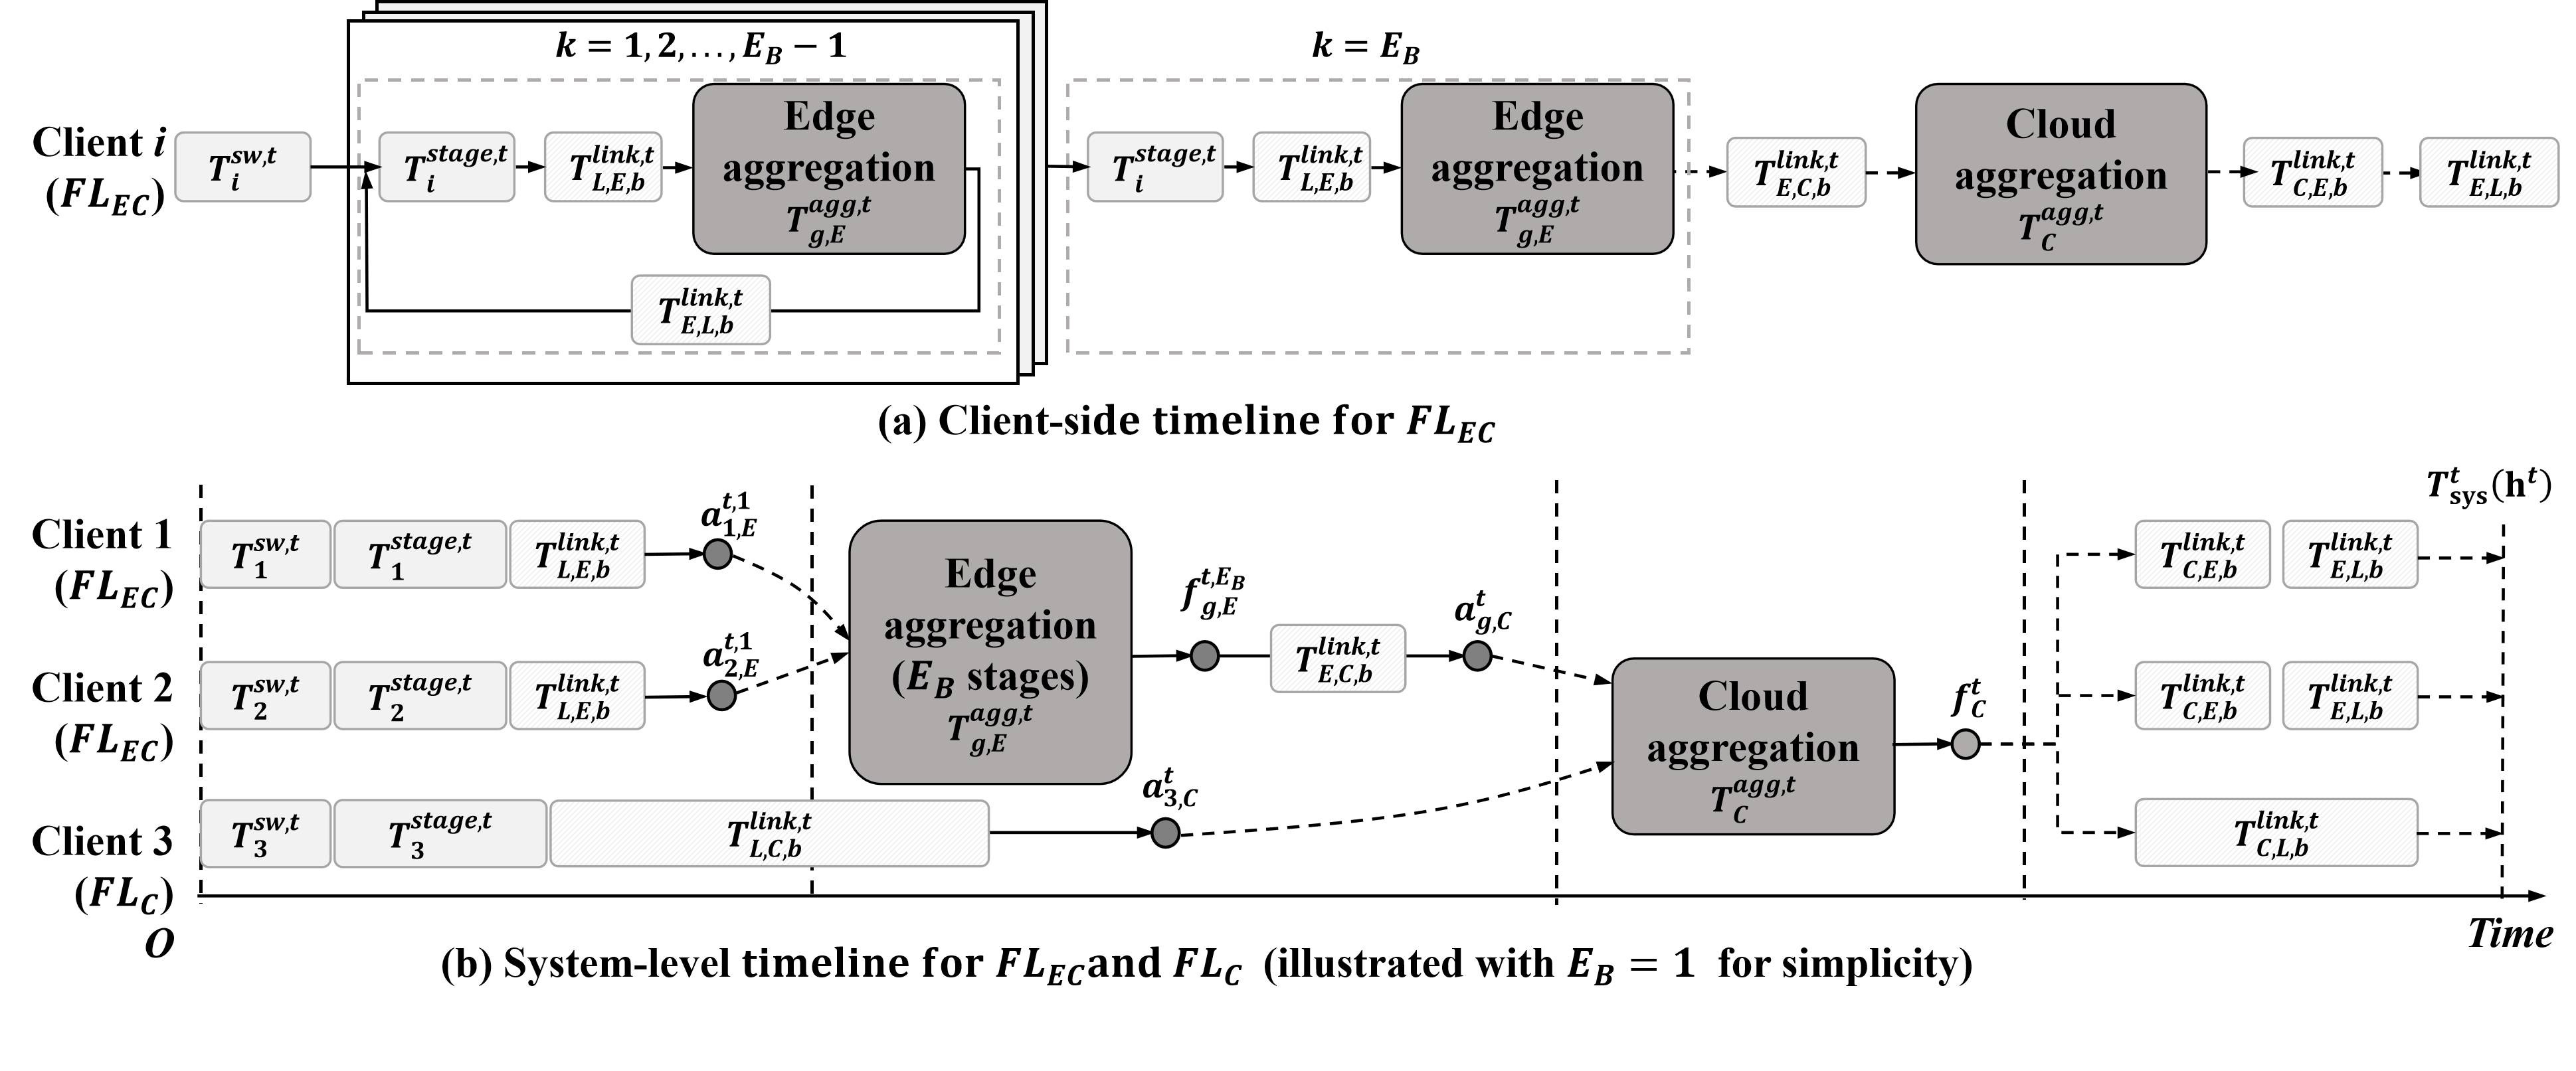
\includegraphics[width=\textwidth]{common_timeline.png}
		\caption{Client-side and system-level latency timelines.
			(a) Client-side execution and communication path 
			for $FL_{EC}$, showing the $E_B$ sequential 
			Edge aggregation stages. 
			(b) System-level synchronization 
			timeline for $FL_{EC}$ and $FL_C$, 
			illustrated with $E_B=1$ for clarity. 
			Cloud aggregation waits for the final 
			$FL_{EC}$ Edge updates and direct $FL_C$ 
			client updates, followed by the required 
			return transmissions. The asynchronous 
			Cloud upload in $FL_E$ is omitted because 
			it does not delay the Cloud-synchronized round.}
		\label{fig:system_timeline}
	\end{figure*}
	
	\textbf{Transmission latency.}
	For a payload \(b\) transmitted from tier \(u\)
	to tier \(v\), let \(S_{u,v,b}^t(h_i)\) denote
	the original payload size under collaboration
	mode \(h_i\). Let \(B_{i,u,v}^t\) denote
	the transmission rate of the link between
	tiers \(u\) and \(v\) for client \(i\) in
	round \(t\), and let \(D_{u,v}^{0}\) denote
	the fixed transmission delay of this link.
	\begin{equation}
		T_{u,v,b}^{\mathrm{link},t}(h_i)
		=
		\frac{S_{u,v,b}^t(h_i)}
		{B_{i,u,v}^t}
		+D_{u,v}^{0}.
		\label{eq:comm_latency}
	\end{equation}
		
	For an aggregated update transmitted from tier
	$u$ to tier $v$, let $S_{u,v,b}^t$ denote
	the payload size and $B_{u,v}^t$ denote
	the corresponding transmission rate.
	The transmission latency is
	\begin{equation}
		T_{u,v,b}^{\mathrm{link},t}
		=
		\frac{S_{u,v,b}^t}{B_{u,v}^t}
		+D_{u,v}^{0}.
	\end{equation}
	
	\textbf{Execution latency.}
	Let \(\tau_{i,L}^t(h)\) denote the estimated
	execution time per local training step for
	client \(i\) under mode \(h\).
	The execution latency is given by
	\begin{equation}
		T_i^{\mathrm{stage},t}(h)
		=
		L_B\tau_{i,L}^t(h),
		\quad
		h\in\{FL_E,FL_{EC},FL_C\}.
		\label{eq:execution_latency}
	\end{equation}
	Transmission and aggregation delays are
	accounted for separately.
	
	\textbf{Reconfiguration latency.}
	Switching collaboration modes may require
	reconfiguring the communication and aggregation
	paths. We model the resulting reconfiguration
	delay as
	\begin{equation}
		T_i^{\mathrm{sw},t}
		=
		\eta_h \mathbb{I}(h_i^t\neq h_i^{t-1}),
		\label{eq:switching_cost}
	\end{equation}
	where \(\eta_h\) denotes the mode switching
	overhead and \(\mathbb{I}(\cdot)\) is the
	indicator function.
	
	\textbf{Path arrival and aggregation.}
	For each candidate mode \(h_i\), the mode flow
	determines the sequence of execution stages
	and payload transmissions leading to the
	relevant aggregation point.
	We calculate update arrival times by
	following this sequence and accounting for
	execution, transmission, and reconfiguration
	delays in their order of occurrence.
	Let \(a_{i,E}^{t,k}(h)\) denote the arrival time
	of client \(i\)'s update at Edge stage \(k\)
	under collaboration mode \(h\). Let \(a_{i,C}^t\)
	denote the arrival time of client \(i\)'s update
	at the Cloud under \(FL_C\).
	
	Given a mode distribution
	$\mathbf h^t=(h_1^t,\ldots,h_N^t)$,
	clients are grouped by their associated Edge
	and selected mode. Let
	\begin{equation}
		\mathcal G_{g,m}^t
		=\{i\mid e(i)=g,\ h_i^t=m\},
		\quad m\in\{FL_E,FL_{EC}\},
		\label{eq:edge_mode_group}
	\end{equation}
	denote the clients assigned to mode $m$
	at Edge $g$. Let \(k\) denote the
	Edge aggregation stage index. For \(FL_E\),
	only one Edge aggregation stage is performed,
	whereas \(FL_{EC}\) consists of \(E_B\)
	sequential Edge aggregation stages.
	
	For \(h\in\{FL_E,FL_{EC}\}\), the update
	arrival time at the first Edge stage is
	\begin{equation}
		a_{i,E}^{t,1}(h)
		=
		T_i^{\mathrm{sw},t}
		+
		T_i^{\mathrm{stage},t}(h)
		+
		T_{L,E,b}^{\mathrm{link},t}(h).
	\end{equation}
	
	For a nonempty Edge group
	$\mathcal G_{g,m}^t$, the completion time
	of aggregation stage $k$ is
	\begin{equation}
		f_{g,E}^{t,k}(m)
		=
		\max_{i\in\mathcal G_{g,m}^t}
		a_{i,E}^{t,k}(m)
		+
		T_{g,E}^{\mathrm{agg},t},
		\label{eq:edge_agg_finish}
	\end{equation}
	where $k=1$ for $FL_E$ and
	$k=1,\ldots,E_B$ for $FL_{EC}$.
	Updates arriving earlier remain buffered
	until all required updates in the same
	aggregation group have arrived.
	
	For \(FL_{EC}\), each subsequent Edge stage
	starts after the aggregated model from the
	previous stage has been returned to the
	clients. The clients then perform another
	local training block and transmit their
	updates to the Edge. Thus, for
	\(k=1,\ldots,E_B-1\), the update arrival
	time at the next stage is
	\begin{equation}
		\begin{aligned}
			a_{i,E}^{t,k+1}(FL_{EC})
			={}&f_{g,E}^{t,k}(FL_{EC})
			+T_{E,L,b}^{\mathrm{link},t}(FL_{EC})\\
			&+T_i^{\mathrm{stage},t}(FL_{EC})
			+T_{L,E,b}^{\mathrm{link},t}(FL_{EC}).
		\end{aligned}
	\end{equation}
	
	For \(FL_E\), the aggregated Edge update is
	forwarded to the Cloud asynchronously after
	the single Edge aggregation stage. This
	transmission does not require clients to wait
	for Cloud aggregation and is excluded from
	the Cloud synchronization latency.
	
	For \(FL_{EC}\), the final Edge update is
	forwarded to the Cloud after the \(E_B\)-th
	Edge aggregation stage. Its arrival time is
	\begin{equation}
		a_{g,C}^t
		=
		f_{g,E}^{t,E_B}(FL_{EC})
		+
		T_{E,C,b}^{\mathrm{link},t}.
	\end{equation}
	
	For \(FL_C\), clients transmit their updates
	directly to the Cloud. The arrival time of
	client \(i\)'s update is
	\begin{equation}
		a_{i,C}^t
		=
		T_i^{\mathrm{sw},t}
		+
		T_i^{\mathrm{stage},t}(FL_C)
		+
		T_{L,C,b}^{\mathrm{link},t}(FL_C).
	\end{equation}
	
	Cloud aggregation waits for the direct client
	updates from $FL_C$ and the final Edge updates
	from $FL_{EC}$. 
	Let $\mathcal G_{EC}^t
	=\{g\mid\mathcal G_{g,FL_{EC}}^t
	\neq\emptyset\}$ denote the Edge servers
	with active $FL_{EC}$ groups. The Cloud aggregation
	completion time is
	\begin{equation}
		\begin{aligned}
			f_C^t
			={}&
			\max\Bigg\{
			\max_{i\in\mathcal D_C^t} a_{i,C}^t,\,
			\max_{g\in\mathcal G_{EC}^t} a_{g,C}^t
			\Bigg\}\\
			&+T_C^{\mathrm{agg},t},
			\label{eq:cloud_agg_finish}
		\end{aligned}
	\end{equation}
	where $\mathcal D_C^t$ denotes the set of
	$FL_C$ clients. The asynchronous uploads
	of $FL_E$ do not affect the Cloud
	synchronization time.
	
	
	The system round latency is measured
	with respect to Cloud synchronization.
	It is determined by the completion times
	of $FL_{EC}$ and $FL_C$ clients, including
	the required return transmissions.
	The asynchronous Cloud uploads of $FL_E$
	do not impose a waiting dependency on
	the Cloud synchronization process.
	The system round latency is therefore
	\begin{equation}
		\begin{aligned}
			T_{\mathrm{sys}}(\mathbf h^t)
			={}&f_C^t+\max\Bigg\{
			\max_{i\in\mathcal D_{EC}^t}
			\Big(
			T_{C,E,b}^{\mathrm{link},t}(h_i^t)
			+
			T_{E,L,b}^{\mathrm{link},t}(h_i^t)
			\Big),\\
			&\qquad
			\max_{i\in\mathcal D_C^t}
			T_{C,L,b}^{\mathrm{link},t}(h_i^t)
			\Bigg\}.
		\end{aligned}
		\label{eq:system_round_latency}
	\end{equation}
	
	Here, $\mathcal D_{EC}^t=\{i\mid h_i^t=FL_{EC}\}$
	and $\mathcal D_C^t=\{i\mid h_i^t=FL_C\}$
	denote the corresponding client sets.
	Clients operating in \(FL_E\) are excluded
	from both sets because they do not wait for
	Cloud aggregation.
	Return delays are evaluated using
	(\ref{eq:comm_latency}), with absent
	return paths excluded from the maximum.
	
	The client-side latency for each collaboration
	mode is defined as
	\begin{equation}
		T_{i,\mathrm{client}}^t(h_i^t)
		=
		\begin{cases}
			f_{g,E}^{t,1}(FL_E)
			+T_{E,L,b}^{\mathrm{link},t}(h_i^t),
			& h_i^t=FL_E,\\[4pt]
			f_C^t
			+T_{C,E,b}^{\mathrm{link},t}(h_i^t)
			+T_{E,L,b}^{\mathrm{link},t}(h_i^t),
			& h_i^t=FL_{EC},\\[4pt]
			f_C^t
			+T_{C,L,b}^{\mathrm{link},t}(h_i^t),
			& h_i^t=FL_C.
		\end{cases}
		\label{eq:client_latency}
	\end{equation}
	
	\subsubsection{Historical Global Update Deviation Modeling}
	\label{sec:learning_cost}
	
	Different collaboration modes involve distinct
	training and aggregation procedures, which may
	result in different update characteristics.
	The historical update deviations of each mode
	are estimated from previous rounds and used
	to evaluate the aggregate deviation signal
	associated with each candidate mode distribution.
	
	\textbf{Cloud aggregation and weights.}
	For a candidate distribution
	$\mathbf h^t=(h_1^t,\ldots,h_N^t)$,
	clients connected to the same Edge and assigned
	the same mode are grouped. Let
	$\mathcal K^t(\mathbf h^t)$ denote the units
	included in the current Cloud aggregation.
	Each $FL_{EC}$ group contributes one final Edge update
	after $E_B$ stages, while each $FL_C$ client
	contributes its own update directly. 
	For $FL_E$, each Edge group sends its
	aggregated update to the Cloud asynchronously.
	The update is included in the Cloud aggregation
	that accepts it, without delaying the current
	synchronization.
	
	Figure~\ref{fig:client_mode_grouping} illustrates
	how mode reassignment changes the grouping structure
	and the resulting Cloud update units.
	From Fig.~\ref{fig:client_mode_grouping}(a) to
	Fig.~\ref{fig:client_mode_grouping}(b), client $l_2$
	switches from $FL_{EC}$ to $FL_C$, while client $l_5$
	switches from $FL_E$ to $FL_{EC}$.
	
	For example, if the two configurations are applied
	in consecutive rounds $t-1$ and $t$, respectively,
	the set of Cloud update units changes from
	\begin{equation}
		\mathcal K^{t-1}(\mathbf h^{t-1})
		=\{k_1,k_2,k_3,k_4,k_5,k_6\}
	\end{equation}
	to
	\begin{equation}
		\mathcal K^t(\mathbf h^t)
		=\{k_1,k_2,k_3,k_4,k_5,k_6,k_7\}.
	\end{equation}
	Here, $k_i$ denotes the $i$th Cloud update unit
	in the corresponding round.
	The units are indexed separately in each round,
	and their composition depends on the client
	mode distribution.
	
	\begin{figure}[t]
		\centering
		\subfloat[Before mode reassignment]{
			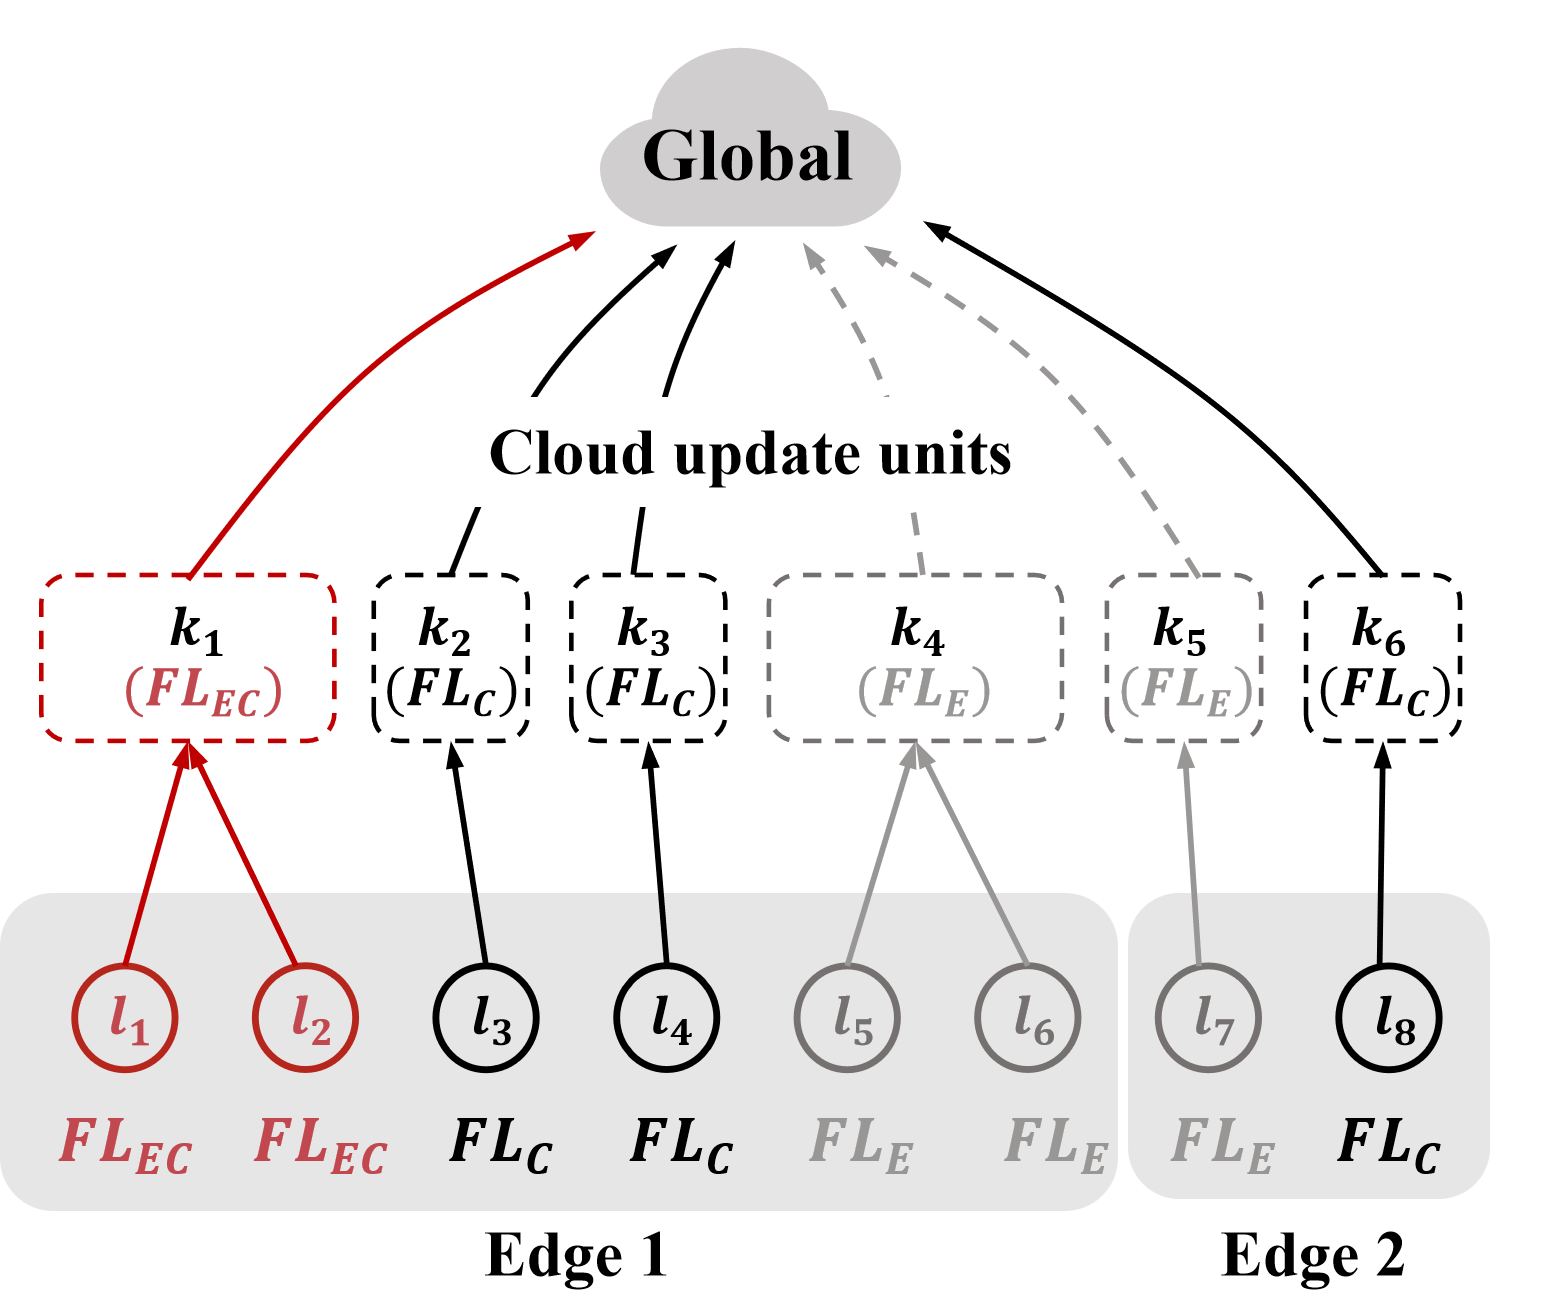
\includegraphics[width=0.90\columnwidth]
			{client_mode_grouping_a.png}
			\label{fig:client_mode_grouping_a}
		}
		
		\subfloat[After mode reassignment]{
			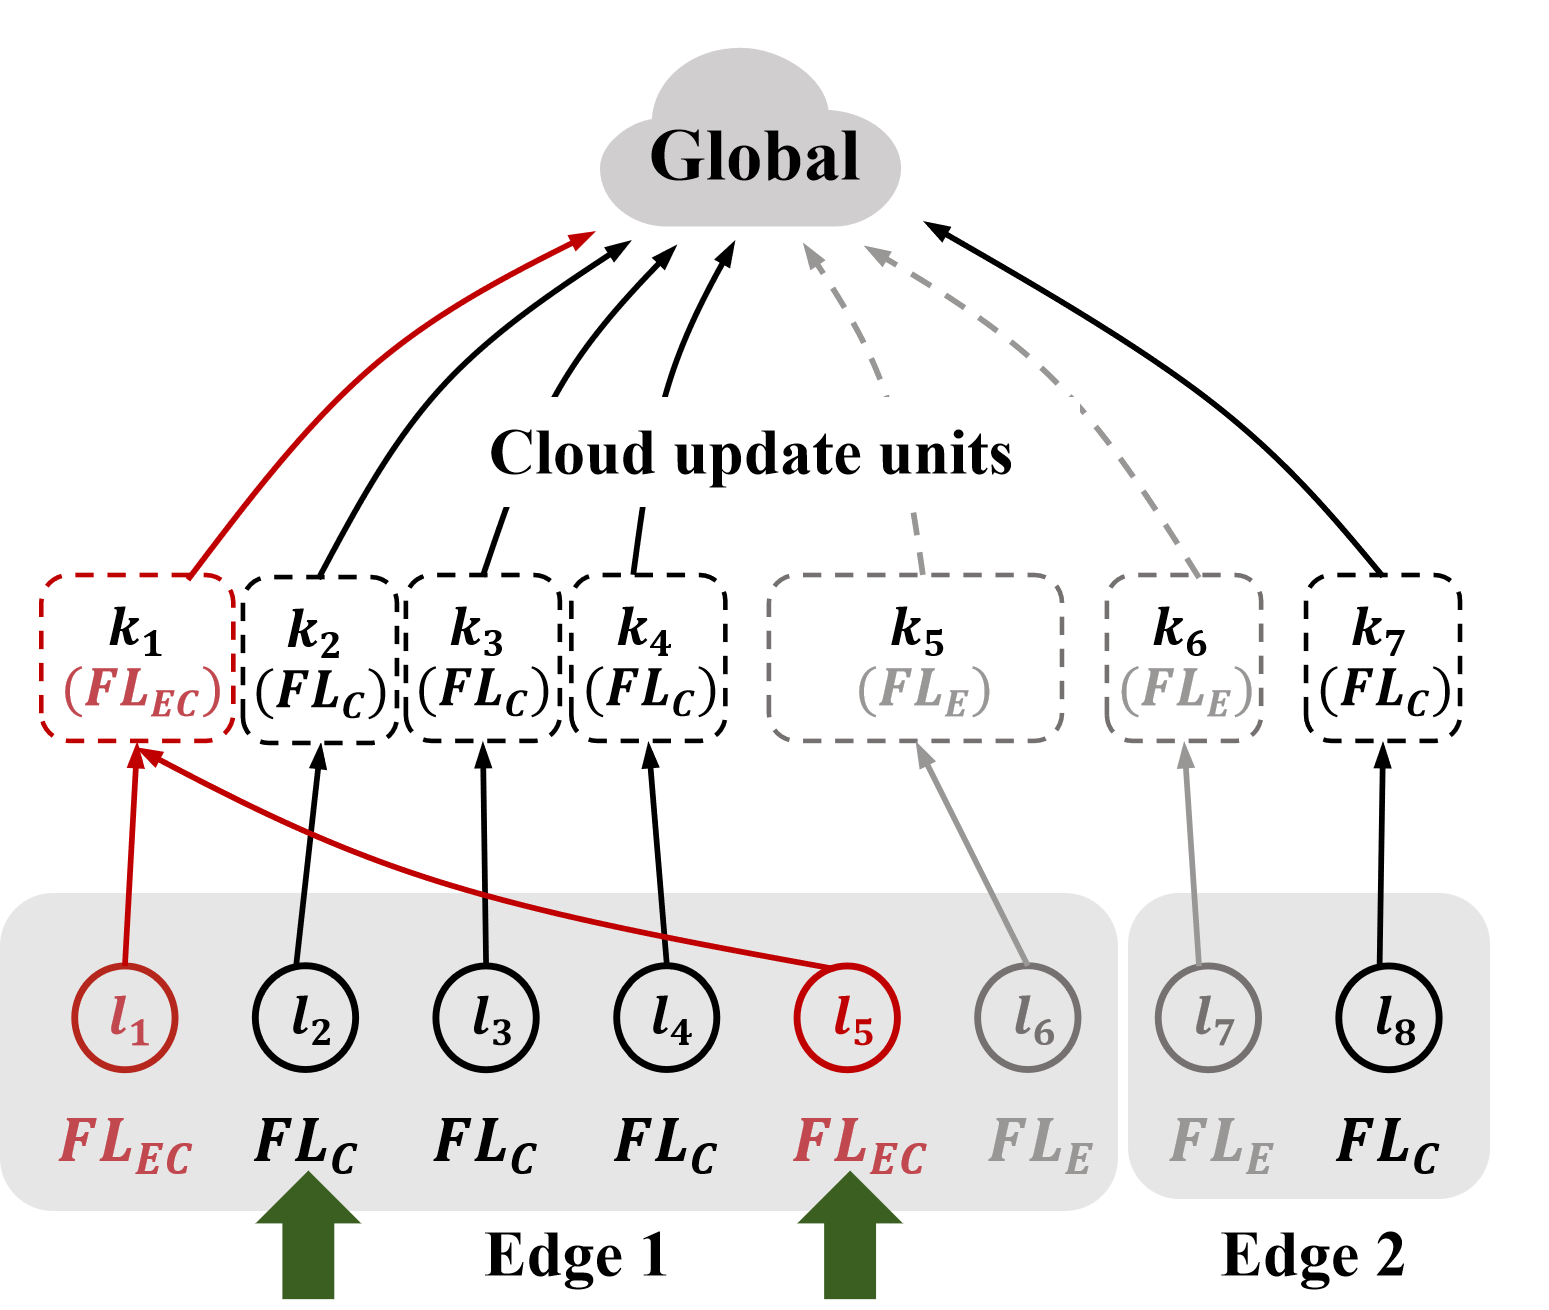
\includegraphics[width=0.90\columnwidth]
			{client_mode_grouping_b.png}
			\label{fig:client_mode_grouping_b}
		}
		
		\caption{Illustration of client grouping and Cloud
			update units under different mode distributions.
			From (a) to (b), client $l_2$ switches from
			$FL_{EC}$ to $FL_C$, while client $l_5$ switches
			from $FL_E$ to $FL_{EC}$. These changes alter
			the grouping structure and the resulting Cloud
			update units.}
		\label{fig:client_mode_grouping}
	\end{figure}
	
	
	Let $n_i$ denote the number of training samples
	of client $i$, and let $\mathcal M_k^t$ denote
	the clients represented by Cloud unit $k$.
	The aggregation weight is calculated as
	\begin{equation}
		\begin{aligned}
			N_k^t
			&=\sum_{i\in\mathcal M_k^t}n_i,\\
			I_k^t(\mathbf h^t)
			&=\frac{N_k^t}
			{\sum_{\ell\in\mathcal K^t(\mathbf h^t)}N_\ell^t}.
		\end{aligned}
		\label{eq:cloud_unit_weights}
	\end{equation}
	
	For example, in Fig.~\ref{fig:client_mode_grouping}(a),
	unit $k_1$ represents clients $l_1$ and $l_2$,
	with $N_{k_1}^{t-1}=n_1+n_2$.
	In Fig.~\ref{fig:client_mode_grouping}(b),
	unit $k_1$ instead represents clients $l_1$
	and $l_5$, with $N_{k_1}^t=n_1+n_5$.
	Meanwhile, client $l_2$ forms an individual
	Cloud update unit $k_2$, with $N_{k_2}^t=n_2$.
	The aggregation weights are determined by
	these sample counts and the total samples
	represented by the accepted Cloud units.
	
	
	\textbf{Historical deviation by mode.}
	Let $\Delta_C^\tau$ denote the Cloud update at round $\tau$.
	The historical global reference is calculated from previous
	Cloud updates as
	\begin{equation}
		v_g^{\tau-1}
		=\gamma_C v_g^{\tau-2}
		+(1-\gamma_C)\Delta_C^{\tau-1},
		\quad 0\leq\gamma_C<1.
		\label{eq:global_ema}
	\end{equation}
	The first available Cloud update is used to initialize
	the reference.
	
	Let $u_{k,\mathrm{DP}}^\tau$ denote the update of unit $k$
	accepted by the Cloud at round $\tau$ after the required
	privacy protection. Only updates allowed under
	Sec.~\ref{sec:privacy_model} are used.
	The deviation of unit $k$ from the historical reference is
	\begin{equation}
		d_k^\tau=u_{k,\mathrm{DP}}^\tau-v_g^{\tau-1}.
		\label{eq:unit_deviation}
	\end{equation}
	Let $\mathcal K_m^\tau$ denote the Cloud units of mode
	$m\in\mathcal H$ included at round $\tau$.
	If this set is not empty, the weighted mean deviation of
	mode $m$ is
	\begin{equation}
		\bar d_m^\tau
		=\frac{\sum_{k\in\mathcal K_m^\tau}I_k^\tau d_k^\tau}
		{\sum_{k\in\mathcal K_m^\tau}I_k^\tau}.
		\label{eq:mode_mean_deviation}
	\end{equation}
	The weighted mean is calculated for each mode across all Edges.
	
	The historical mean deviation of each mode is estimated
	using an exponential moving average (EMA):
	\begin{equation}
		\widehat d_m^t
		=\gamma_d\widehat d_m^{t-1}
		+(1-\gamma_d)\bar d_m^{t-1},
		\quad 0\leq\gamma_d<1.
		\label{eq:mode_deviation_ema}
	\end{equation}
	The first available mean deviation is used to initialize
	the estimate. If no new data are available, the previous
	estimate is retained.
	As clients switch modes between rounds, the set of clients
	assigned to the same mode at each Edge may change.
	Therefore, the mean deviation is estimated for each mode
	rather than for a fixed group of clients.
	
	\textbf{Update deviation score.}
	For each candidate mode distribution $\mathbf h^t$,
	the Cloud units and their aggregation weights are determined.
	The historical deviation contributions are aggregated
	and combined with the global reference as follows:
	\begin{equation}
		\widehat U_C^t(\mathbf h^t)
		=v_g^{t-1}
		+\sum_{k\in\mathcal K^t(\mathbf h^t)}
		I_k^t(\mathbf h^t)\widehat d_{m(k)}^t,
		\label{eq:predicted_cloud_update}
	\end{equation}
	Here, $m(k)$ denotes the collaboration mode
	of Cloud update unit $k$.
	For example, in Fig.~\ref{fig:client_mode_grouping}(b),
	$m(k_1)=FL_{EC}$ and $m(k_2)=FL_C$.
	Their contributions to the aggregate deviation
	are weighted by $I_{k_1}^t(\mathbf h^t)$
	and $I_{k_2}^t(\mathbf h^t)$, respectively.
	The update deviation score measures the normalized
	squared magnitude of the aggregate historical
	deviation contribution:
	\begin{equation}
		J^t(\mathbf h^t)
		=\frac{\left\|\widehat U_C^t(\mathbf h^t)
			-v_g^{t-1}\right\|_2^2}
		{\left\|v_g^{t-1}\right\|_2^2+\varepsilon_J},
		\quad\varepsilon_J>0.
		\label{eq:j_learn_estimate}
	\end{equation}
	A larger $J^t(\mathbf h^t)$ indicates a greater
	historical aggregate update deviation under
	the candidate mode distribution.
	Therefore, larger values of $J^t(\mathbf h^t)$
	are preferred to prioritize mode distributions
	with more pronounced historical update
	characteristics.
	The system latency is also considered to
	balance the historical aggregate update
	deviation score and the execution overhead.
	
	\subsection{Finite Candidate Joint Selection}
	\label{sec:global_optimization}
	
	
	Let $P_j$ denote a candidate mode distribution,
	where $j=0,\ldots,M-1$ and $M$ is the number
	of candidate distributions considered.
	Each candidate specifies the proportions
	of clients assigned to $(FL_E,FL_{EC},FL_C)$.
	
	For each candidate $P_j$, let
	$\mathbf h_j^t=\Psi^t(P_j)$
	denote the corresponding client mode assignment
	in round $t$, where $\Psi^t$ represents
	the assignment procedure applied at each Edge.
	
	
	Let $\mathcal F_{\mathrm{sys}}^t$ denote the set
	of client mode assignments satisfying the
	resource, privacy, and system admission
	constraints in round $t$.
	The feasible candidate set is defined as
	\begin{equation}
		\mathcal C^t
		=
		\left\{
		\mathbf h_j^t \mid
		0\leq j<M,\;
		\mathbf h_j^t\in\mathcal F_{\mathrm{sys}}^t
		\right\}.
		\label{eq:feasible_candidates}
	\end{equation}
	
	The search complexity is $O(M)$,
	as at most $M$ candidate distributions
	are considered for joint utility maximization.
	
	The candidate set can be extended by considering
	additional mode distributions.
	For experimental evaluation, five candidate
	mode distributions are considered, with $M=5$.
	Their proportions for $(FL_E,FL_{EC},FL_C)$
	are specified as
	\[
	\begin{array}{ll}
		P_0=(0.30,0.30,0.40), & P_1=(0.50,0.25,0.25),\\
		P_2=(0.25,0.50,0.25), & P_3=(0.25,0.25,0.50),\\
		P_4=(0.40,0.40,0.20). &
	\end{array}
	\]
	
	The specified proportions are applied separately
	to the clients associated with each Edge.
	For each candidate, the number of clients
	assigned to each mode is obtained by rounding
	the corresponding proportion and adjusting
	the resulting counts to match the total
	number of clients at that Edge.
	
	For each feasible assignment
	$\mathbf h_j^t\in\mathcal C^t$,
	the historical update deviation score
	$J^t(\mathbf h_j^t)$ and system latency
	$T_{\mathrm{sys}}(\mathbf h_j^t)$
	are evaluated.
	All candidates are evaluated using the
	historical statistics and system conditions
	available in round $t$.
	
	Since the two quantities have different scales,
	their values are normalized among the feasible
	candidates in each round.
	Let $J_{\min}^t$ and $J_{\max}^t$ denote the
	minimum and maximum values of $J^t$.
	Similarly, $T_{\min}^t$ and $T_{\max}^t$
	denote the minimum and maximum system latencies.
	
	The joint utility is defined as
	\begin{equation}
		\begin{aligned}
			U^t(\mathbf h^t;\lambda)
			={}&\lambda
			\frac{J^t(\mathbf h^t)-J_{\min}^t}
			{J_{\max}^t-J_{\min}^t}\\
			&+(1-\lambda)
			\frac{T_{\max}^t-T_{\mathrm{sys}}(\mathbf h^t)}
			{T_{\max}^t-T_{\min}^t},
		\end{aligned}
		\label{eq:joint_utility}
	\end{equation}
	where $0\leq\lambda\leq1$ controls the relative
	importance of the historical deviation
	contribution and system latency.
	A normalized value of $0.5$ is used when
	the corresponding maximum and minimum are equal.
	
	A larger $J^t(\mathbf h^t)$ is preferred
	to favor stronger historical aggregate
	deviation contributions.
	A smaller $T_{\mathrm{sys}}(\mathbf h^t)$
	is preferred to reduce system execution time.
	Both preferences are therefore represented
	by larger normalized values in the joint utility.
	
	The mode distribution is selected by
	\begin{equation}
		\mathbf h^{t,\ast}
		\in
		\arg\max_{\mathbf h^t\in\mathcal C^t}
		U^t(\mathbf h^t;\lambda).
		\label{eq:joint_selection}
	\end{equation}
	If multiple candidates achieve the same
	maximum utility, the candidate with the
	smallest index is selected.
	
	\section{Algorithm}
	\label{sec:algorithm}
	
	Algorithm~\ref{alg:selection} presents the
	dynamic collaboration mode selection procedure,
	and the main symbols are summarized in
	Table~\ref{tab:algorithm_notation}.
	At each mode selection step, at most $M$
	candidate distributions are evaluated
	based on their feasibility, historical
	deviation contribution, and system latency.
	The candidate search complexity is $O(M)$
	in terms of the number of candidate evaluations.
	
	\begin{table}[t]
		\centering
		\caption{Notation Used in Algorithm~\ref{alg:selection}}
		\label{tab:algorithm_notation}
		\small
		\setlength{\tabcolsep}{4pt}
		\begin{tabular}{p{0.37\columnwidth}p{0.54\columnwidth}}
			\hline
			\textbf{Symbol} & \textbf{Description} \\
			\hline
			$M$ & Number of candidate mode distributions. \\
			$P_j$ & Candidate mode distribution indexed by $j$. \\
			$S_P$ & Mode selection period. \\
			$\mathcal F_{\mathrm{sys}}^t$ &
			Set of system feasible mode distributions. \\
			$\mathcal C^t$ &
			Set of feasible candidate distributions in round $t$. \\
			$\mathbf h^{t,\ast}$ &
			Selected mode distribution in round $t$. \\
			$J^t(\mathbf h^t)$ &
			Historical aggregate deviation contribution. \\
			$T_{\mathrm{sys}}(\mathbf h^t)$ &
			System latency under distribution $\mathbf h^t$. \\
			$U^t(\mathbf h^t;\lambda)$ &
			Joint utility for candidate selection. \\
			\hline
		\end{tabular}
	\end{table}
	
	\begin{breakablealgorithm}
		\caption{Dynamic Collaboration Mode Selection}
		\label{alg:selection}
		\small
		\begin{algorithmic}[1]
			\REQUIRE Round $t$, candidate distributions
			$\{P_j\}_{j=0}^{M-1}$,
			strategy period $S_P$,
			utility weight $\lambda$,
			hysteresis threshold $\theta_H$,
			previous candidate index $j_{t-1}$,
			system state, privacy ledger,
			and historical statistics
			\ENSURE Selected mode distribution
			$\mathbf h^{t,\ast}$ or \textsc{skip}
			
			\IF{$t\leq 5$}
			\STATE $\mathbf h_0^t\leftarrow\Psi^t(P_0)$
			
			\IF{$\mathbf h_0^t\notin\mathcal F_{\mathrm{sys}}^t$}
			\STATE \textbf{return} \textsc{skip}
			\ENDIF
			
			\STATE \textbf{return} $\mathbf h_0^t$
			\ENDIF
			
			\IF{$t>1$,
				$\operatorname{mod}(t-1,S_P)\neq0$,
				and $\mathbf h^{t-1,\ast}
				\in\mathcal F_{\mathrm{sys}}^t$}
			
			\STATE $\mathbf h^{t,\ast}
			\leftarrow\mathbf h^{t-1,\ast}$
			
			\ELSE
			
			\STATE Construct $\mathcal C^t$
			using \eqref{eq:feasible_candidates}
			
			\IF{$\mathcal C^t=\emptyset$}
			\STATE \textbf{return} \textsc{skip}
			\ENDIF
			
			\STATE Freeze $v_g^{t-1}$ and
			$\{\widehat d_m^t\}_{m\in\mathcal H}$
			
			
			\FORALL{$\mathbf h_j^t\in\mathcal C^t$}
			
			\STATE Evaluate
			$J^t(\mathbf h_j^t)$
			using \eqref{eq:j_learn_estimate}
			
			\STATE Evaluate
			$T_{\mathrm{sys}}(\mathbf h_j^t)$
			using \eqref{eq:system_round_latency}
			
			\ENDFOR
			
			\STATE Determine
			$J_{\min}^t$, $J_{\max}^t$,
			$T_{\min}^t$, and $T_{\max}^t$
			from all feasible candidates
			
			\FORALL{$\mathbf h_j^t\in\mathcal C^t$}
			
			\STATE Compute
			$U^t(\mathbf h_j^t;\lambda)$
			using \eqref{eq:joint_utility}
			
			\ENDFOR			
			
			
			\STATE Select $\mathbf h^{t,\ast}$
			using \eqref{eq:joint_selection}
			
			\STATE Resolve utility ties
			by selecting the candidate
			with the smallest index $j$
			
			\IF{$\theta_H>0$ and $t>1$}
			
			\IF{$\mathbf h_{j_{t-1}}^t\in\mathcal C^t$}
			
			\IF{$U^t(\mathbf h^{t,\ast};\lambda)
				-U^t(\mathbf h_{j_{t-1}}^t;\lambda)
				\leq\theta_H$}
			
			\STATE $\mathbf h^{t,\ast}
			\leftarrow\mathbf h_{j_{t-1}}^t$
			
			\ENDIF
			\ENDIF
			\ENDIF
			
			\ENDIF
			
			\STATE \textbf{return} $\mathbf h^{t,\ast}$
			
		\end{algorithmic}
	\end{breakablealgorithm}
	
	\section{Experiments}
	\label{sec:experiment}
	
	The experiments test whether the proposed dynamic collaboration
	mode selection method, which jointly considers the historical
	aggregate deviation contribution $J^t(\mathbf h^t)$ and system
	latency $T_{\mathrm{sys}}(\mathbf h^t)$, achieves a more favorable
	tradeoff between test loss and cumulative system latency than fixed
	collaboration mode distributions. Five fixed strategies based on
	$P_0,\ldots,P_4$ are compared with seven dynamic strategies: three
	Greedy variants with $\lambda\in\{0.25,0.50,0.75\}$, Maximum $J$,
	Minimum $T$, Hysteresis, and Periodic selection. The comparisons
	cover convergence, communication and computation costs, and
	candidate selection, with particular attention to the effects of
	Hysteresis and Periodic selection on mode switching.
	
	\subsection{Experimental Setup}
	\label{sec:exp_setup}
	
	\textbf{Data and training.}
	Fashion MNIST contains 60,000 training images and 10,000 test images.
	To simulate heterogeneous data distributions, the training samples
	of each class are allocated to ten Edge servers using a Dirichlet
	distribution with concentration parameter $\alpha=0.5$.
	Each Edge server then distributes its assigned samples among
	ten clients. A LeNet 5 model is trained for 100 global rounds.
	The training parameters and collaboration mode configurations
	are summarized in Table~\ref{tab:experimental_setup}.
	The reverse links are assumed to have the same nominal transmission rates and fixed delays as the corresponding forward links.
	
	\textbf{System conditions.}
	To model differences in client computing capabilities,
	each client is assigned a computation factor sampled from
	$\mathcal U(0.5,2.0)$ and held constant across rounds.
	The local computation time per step is 0.1 s multiplied
	by this factor, while the client compute capacity is
	2.0 divided by the same factor.
	Client memory is independently assigned by multiplying
	32 MB by a fixed draw from $\mathcal U(0.5,2.0)$.
	All 100 clients satisfy the resource requirements
	and participate in every training round.
	The same client population is used across strategies
	to compare different collaboration mode distributions.
	The system resource settings are listed in
	Table~\ref{tab:experimental_setup}.
	
	\textbf{System latency.}
	Different collaboration modes involve different
	computation, communication, and aggregation processes,
	which lead to different system latencies.
	To capture these differences, an event based
	simulation is used to model the execution
	timeline of each collaboration mode.
	All strategies are evaluated using the same
	system conditions and timing rules to provide
	a consistent comparison of system efficiency.
	Communication latency is calculated using
	Eq.~\eqref{eq:comm_latency}, while local execution,
	Edge aggregation, Cloud aggregation, and mode
	reconfiguration follow
	Eqs.~\eqref{eq:execution_latency},
	\eqref{eq:edge_agg_finish},
	\eqref{eq:cloud_agg_finish}, and
	\eqref{eq:switching_cost}, respectively.
	The transmission rates, link delays, and
	other latency parameters are summarized in
	Table~\ref{tab:experimental_setup}.
	
	\textbf{Privacy configuration.}
	Local training applies per example gradient clipping
	with $C=1.0$, followed by Gaussian noise addition
	at each local update step.
	Under replacement adjacency, the sensitivity is
	$2C$, and the noise standard deviation is
	$2C\sigma$.
	Privacy expenditure is tracked using an RDP
	accountant without sampling amplification.
	The privacy parameters are summarized in
	Table~\ref{tab:experimental_setup}.
	The noise multiplier is calibrated according
	to the selected collaboration mode and the
	remaining lifetime privacy budget, as specified
	in \eqref{eq:noise_calibration}. In the reported
	experimental configuration, the representative
	values are approximately $9.803$ for $FL_E$
	and $FL_C$, and $16.979$ for $FL_{EC}$.
	
	\begin{table}[t]
		\centering
		\caption{Experimental configuration.}
		\label{tab:experimental_setup}
		\scriptsize
		\setlength{\tabcolsep}{4pt}
		\renewcommand{\arraystretch}{1.12}
		\begin{tabularx}{\columnwidth}{@{}lX@{}}
			\toprule
			\textbf{Parameter} & \textbf{Configuration} \\
			\midrule
			\multicolumn{2}{@{}l}{\textit{Data and training}} \\
			Dataset & Fashion MNIST (60,000 training, 10,000 test) \\
			Model & LeNet 5 \\
			Topology & 100 clients, 10 Edge servers \\
			Data heterogeneity & Dirichlet distribution, $\alpha=0.5$ \\
			Global rounds & 100 \\
			Local optimization & DP SGD, batch size 64, learning rate 0.05 \\
			Local steps & 2 per training stage \\
			Mode stages & $FL_E$: 1, $FL_{EC}$: 3, $FL_C$: 1 \\
			\midrule
			\multicolumn{2}{@{}l}{\textit{System conditions}} \\
			Local computation & 0.1 s per step, factor $\mathcal U(0.5,2.0)$ \\
			Client memory & 32 MB, factor $\mathcal U(0.5,2.0)$ \\
			Client participation & All 100 clients per round \\
			\midrule
			\multicolumn{2}{@{}l}{\textit{System latency}} \\
			Link rates & $L\to E$: 5.0, $L\to C$: 2.2, $E\to C$: 8.0 MB/s \\
			Rate variation & $\mathcal U(0.75,1.25)$ per client and round \\
			Link delays & $L\to E$: 0.015, $L\to C$: 0.04, $E\to C$: 0.01 s \\
			Edge aggregation & 0.02 s per group and stage \\
			Cloud aggregation & 0.04 s per aggregation \\
			Mode switching & 0.02 s per changed client \\
			\midrule
			\multicolumn{2}{@{}l}{\textit{Privacy configuration}} \\
			Clipping norm & $C=1.0$ \\
			Noise multiplier & Mode and budget dependent;
			$FL_E$, $FL_C$: $\sigma\approx9.803$;
			$FL_{EC}$: $\sigma\approx16.979$ \\
			Privacy budget & $\epsilon\leq8$, $\delta=10^{-5}$ \\
			\bottomrule
		\end{tabularx}
	\end{table}
	
	\subsection{Comparison Strategies and Evaluation Metrics}
	\label{sec:exp_strategies_metrics}
	
	\textbf{Main comparison.}
	All fixed and dynamic strategies use the five candidate
	distributions $P_0,\ldots,P_4$ defined in
	Sec.~\ref{sec:global_optimization}.
	Each fixed strategy retains one candidate throughout
	training, while dynamic strategies select candidates
	according to the joint utility or its individual
	objective components.
	The Greedy variants maximize
	$U^t(\mathbf h^t;\lambda)$ with
	$\lambda\in\{0.25,0.50,0.75\}$,
	while Maximum $J$ and Minimum $T$ prioritize
	the respective objective components.
	Hysteresis and Periodic selection use
	$\lambda=0.50$ with additional restrictions
	on reconfiguration.
	Hysteresis requires a utility improvement
	greater than 0.05 before switching candidates,
	whereas Periodic selection allows a new
	decision every five rounds.
	These strategies examine how restrictions
	on mode switching affect learning performance
	and system latency.
	
	\textbf{Pure mode references.}
	Three pure mode strategies are considered, where
	all clients use the same collaboration mode
	throughout training: $FL_E$, $FL_{EC}$, or $FL_C$.
	These strategies are evaluated separately from
	the five candidate distributions to compare
	the learning performance and system costs of
	different collaboration modes.
	
	All dynamic strategies first execute $P_0$ for five rounds.
	Its relatively balanced proportions allow historical update
	information to be collected from all three collaboration modes.
	Candidate selection then begins in round 6 using the
	accumulated historical statistics.
	
	\textbf{Metrics.}
	Learning performance is evaluated using test loss
	and test accuracy. System efficiency is measured
	by cumulative system latency, total communication
	volume in MB, and the number of local training steps.
	Candidate changes and client mode changes are recorded
	to evaluate mode switching behavior.
	\subsection{Learning Performance and Efficiency}
	\label{sec:exp_convergence}
	\label{sec:main_comparison}
	The five fixed candidate distributions are first compared by test loss and cumulative system latency. The values of the historical aggregate deviation contribution \(J\) and system latency are then compared for feasible candidates at the first online decision. Finally, the dynamic selection strategies are evaluated over training. For the main experiments, results are reported
	as means across seeds 42, 43, and 44, with
	shaded bands or error bars indicating one
	sample standard deviation.
	\subsubsection{Fixed Candidate Learning Performance}
	Figure~\ref{fig:fixed_loss_vs_cumulative_latency} compares
	Fixed $P_0$ to Fixed $P_4$ by test loss and cumulative system
	latency to assess their learning progress relative to the
	simulated time required.
	The mean final losses increase in the order
	$P_2$, $P_4$, $P_0$, $P_1$, and $P_3$.
	Fixed $P_2$ obtains the lowest mean final loss,
	$1.1992\pm0.0188$, and the highest mean
	accuracy over rounds 91--100 among the
	fixed strategies, $54.97\pm0.78\%$.
	\begin{figure}[t]
		\centering
		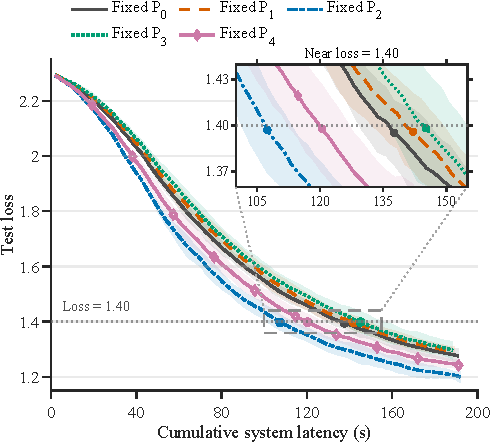
\includegraphics[width=\columnwidth]
		{experiment_fixed_loss_vs_cumulative_T.pdf}
		\caption{Test loss versus cumulative system latency
			for fixed strategies. Inset circles mark the
			first recorded mean loss at or below 1.40.}
		\label{fig:fixed_loss_vs_cumulative_latency}
	\end{figure}
	
	The inset highlights the latency differences near loss 1.40.
	The mean curves first reach this level in the order
	$P_2$, $P_4$, $P_0$, $P_1$, and $P_3$,
	as summarized in Table~\ref{tab:fixed_loss_140}.
	Fixed $P_2$ reaches this reference level at 107.45 s,
	compared with 137.56 s for Fixed $P_0$,
	a reduction of approximately 21.9\%.		
	\begin{table}[t]
		\centering
		\caption{Client mode proportions and cumulative latency
			at the circled points in
			Fig.~\ref{fig:fixed_loss_vs_cumulative_latency}.
			Latency is reported as mean $\pm$ sample standard deviation.}
		\label{tab:fixed_loss_140}
		\footnotesize
		\setlength{\tabcolsep}{0pt}
		\begin{tabular}{@{}
				>{\raggedright\arraybackslash}p{0.22\columnwidth}
				>{\centering\arraybackslash}p{0.11\columnwidth}
				>{\centering\arraybackslash}p{0.13\columnwidth}
				>{\centering\arraybackslash}p{0.11\columnwidth}
				>{\raggedleft\arraybackslash}p{0.33\columnwidth}
				@{}}
			\toprule
			Candidate & $FL_E$ & $FL_{EC}$ & $FL_C$
			& \mbox{Cumulative latency (s)} \\
			\midrule
			Fixed $P_0$ & 30\% & 30\% & 40\% & $137.56\pm1.55$ \\
			Fixed $P_1$ & 50\% & 25\% & 25\% & $142.07\pm1.13$ \\
			Fixed $P_2$ & 25\% & 50\% & 25\% & $107.45\pm0.87$ \\
			Fixed $P_3$ & 25\% & 25\% & 50\% & $145.10\pm4.30$ \\
			Fixed $P_4$ & 40\% & 40\% & 20\% & $120.38\pm1.54$ \\
			\bottomrule
		\end{tabular}
	\end{table}	
	These results show that $P_2$ and $P_4$, which assign
	50\% and 40\% of clients to $FL_{EC}$, respectively,
	achieve lower mean final losses than the other fixed
	configurations.
	However, these configurations also execute more local
	training steps.
	Fixed $P_2$ and $P_4$ execute 400 and 360 steps per round,
	compared with 320 for $P_0$ and 300 for $P_1$ and $P_3$.
	Their results therefore reflect both the collaboration
	configuration and the amount of training performed.
	\subsubsection{Candidate Scores and Training Tradeoffs}
	Figure~\ref{fig:round6_candidate_jt} compares candidate
	scores with subsequent learning performance from a
	common training state.
	After five rounds of $P_0$,
	all five candidates are evaluated using the same
	model and historical information. Each candidate is
	then applied separately in rounds 6 to 10.
	This preliminary experiment uses seed 42,
	with results obtained from a single run
	for each candidate.
	The inset shows the corresponding $J$ and system
	latency $T$, while the main plot shows the subsequent
	test loss.
	
	\begin{figure}[t]
		\centering
		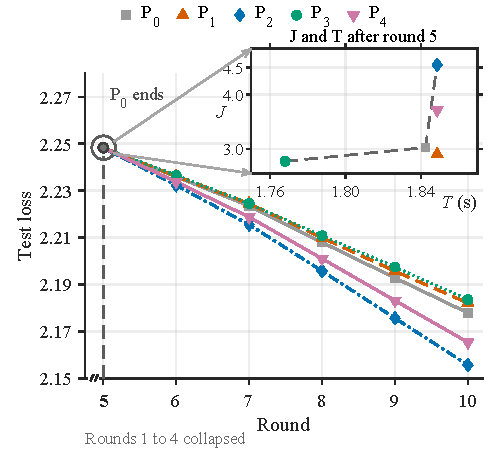
\includegraphics[width=0.96\columnwidth]{experiment_pilot_loss_JT_folded.pdf}
		\caption{Candidate scores and subsequent test loss following five
			common rounds of $P_0$. The circled point marks the end of round 5.
			Each continuation uses one candidate in rounds 6 to 10. The inset
			shows historical deviation contribution $J$ and system latency
			$T$ in seconds, evaluated at the common round 5 state. Its dashed
			line connects the nondominated candidate scores. Results are obtained using seed 42.}
		\label{fig:round6_candidate_jt}
	\end{figure}	
	
	The inset identifies $P_3$, $P_0$, and $P_2$ as
	nondominated candidates at the common decision state.
	Among them, $P_2$ provides the largest $J$, whereas
	$P_3$ has the smallest system latency $T$.
	$P_0$ has intermediate values of both objectives,
	offering a compromise between historical deviation
	contribution and system latency.
	
	The main plot shows the subsequent learning outcomes
	when these candidates are retained for five rounds.
	From round 5 to round 10, the loss reductions for
	$P_2$, $P_0$, and $P_3$ are 0.0926, 0.0704, and
	0.0648, respectively, following the same ordering
	as their initial $J$ values.
	Meanwhile, the recorded cumulative system latencies
	at round 10 are 18.8601, 18.8527, and 18.4668 s,
	respectively. Thus, $P_2$ achieves the largest loss
	reduction, while $P_3$ requires the least system time.
	This ordering is consistent with the fixed
	strategy results in
	Fig.~\ref{fig:fixed_loss_vs_cumulative_latency}, where $P_2$ achieves the lowest final loss
	among the fixed candidates. These observations provide preliminary empirical support for using
	$J$ as an indicator of potential learning progress when comparing candidate mode distributions.
	
	\subsection{Dynamic Selection and Switching Control}
	\label{sec:exp_joint_selection}
	\label{sec:reconfiguration_behavior}	
	The preceding comparison motivates using $J$
	together with system latency $T$ in the joint
	utility $U$ defined in \eqref{eq:joint_utility}.
	The values $\lambda=0.25$, $0.50$, and $0.75$
	represent a stronger preference for lower latency,
	equal weighting of the two normalized terms,
	and a stronger preference for historical deviation
	contribution, respectively.
	Starting from round 6, Greedy evaluates the feasible
	candidates in every round and selects the distribution
	with the highest current $U$, allowing candidate
	choices to adapt as training progresses.
	This subsection examines how $\lambda$ influences
	the learning and latency tradeoffs, and how
	hysteresis and periodic updates regulate
	mode switching.
	\subsubsection{Effect of the Joint Utility Weight}
	
	Figure~\ref{fig:dynamic_loss_vs_cumulative_latency} examines how
	the preference between historical deviation contribution and system
	latency affects learning efficiency. The three Greedy strategies
	share the same five rounds of $P_0$ initialization within each seed
	and differ in the weight used for subsequent candidate selection.
	
	\begin{figure}[t]
		\centering
		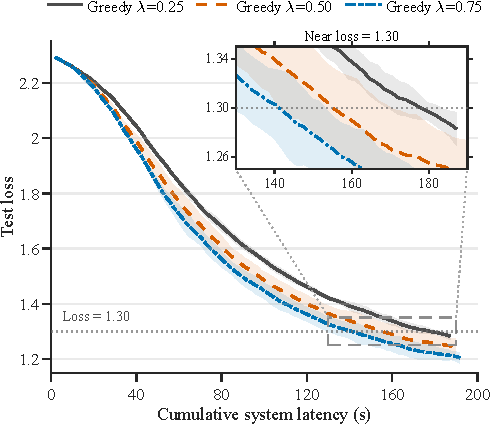
\includegraphics[width=0.96\columnwidth]{experiment_greedy_weights_loss_vs_cumulative_T.pdf}
		\caption{Test loss versus cumulative system latency
			for the three Greedy weights. Curves show mean
			loss against mean cumulative latency at
			matching rounds across three seeds.
			The inset enlarges the region near loss 1.30.}
		\label{fig:dynamic_loss_vs_cumulative_latency}
	\end{figure}
	
	The curves show faster mean loss reduction as $\lambda$ increases over the three tested values, with the inset highlighting their separation near loss 1.30. Greedy $\lambda=0.25$, $0.50$, and $0.75$ first reach this threshold at mean rounds $94.7\pm3.8$, $83.0\pm7.8$, and $74.0\pm6.0$, with mean cumulative latencies	$177.28\pm10.03$, $157.60\pm16.21$, and $141.95\pm11.82$ s, respectively. Thus, a stronger preference for lower candidate latency in each	round does not necessarily reduce the cumulative time needed to reach a given loss. Among the tested weights, $\lambda=0.75$ provides the earliest mean crossing of loss 1.30.
	
	\subsubsection{Objective Preferences and Switching Control}
	
	Figure~\ref{fig:dynamic_controls_loss_vs_cumulative_latency}
	compares Greedy $\lambda=0.50$ with Maximum $J$ and Minimum $T$
	to examine the learning consequences of emphasizing either objective
	alone. Hysteresis and Periodic retain $\lambda=0.50$ while regulating
	when candidate changes are applied, allowing their learning and
	latency outcomes to be compared with the same Greedy reference.
	
	\begin{figure}[t]
		\centering
		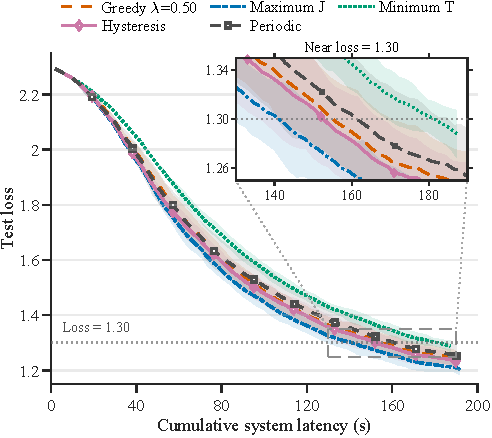
\includegraphics[width=0.96\columnwidth]{experiment_objectives_switching_loss_vs_cumulative_T.pdf}
		\caption{Test loss versus cumulative system latency
			for the objective and switching controls, with
			Greedy $\lambda=0.50$ as the reference.
			The inset enlarges the region near loss 1.30.}
		\label{fig:dynamic_controls_loss_vs_cumulative_latency}
	\end{figure}
	
	Maximum $J$ follows the same loss and simulated latency trajectory as Greedy $\lambda=0.75$.The decision records show that Maximum $J$ and Greedy $\lambda=0.75$ both select $P_2$ in all 95 decisions after the common prefix in all three seeds. For each recorded state, their choices satisfy the respective	maximum $J$ or maximum utility rule among the feasible members of the five candidate set. 
	
	Hysteresis remains close to the Greedy $\lambda=0.50$ reference,
	while Periodic shows slower mean loss reduction near the threshold.
	Hysteresis and Periodic reach loss 1.30 in all three seeds at mean
	rounds $80.0\pm8.9$ and $86.0\pm12.1$, respectively.
	The corresponding switching behavior is
	examined in Fig.~\ref{fig:selection_switching}.
	Hysteresis reduces mode changes while
	maintaining learning performance comparable
	to Greedy $\lambda=0.50$, whereas Periodic
	further reduces switching but exhibits slower
	loss reduction near the threshold.
	
	\subsubsection{Mode Selection and Switching}
	Figure~\ref{fig:selection_switching} examines how objective
	preferences affect candidate choices and how switching controls
	regulate reconfiguration activity. After the common initialization,
	Greedy $\lambda=0.25$ and Minimum $T$ mainly select $P_1$ and $P_3$,
	although their relative frequencies differ across seeds.
	Greedy $\lambda=0.75$ and Maximum $J$ consistently select $P_2$
	throughout the remaining 95 rounds in all three seeds.
	Greedy $\lambda=0.50$ selects $P_2$ most frequently in each seed
	while also selecting other candidates.
	
	The switching controls substantially reduce reconfiguration
	activity relative to Greedy $\lambda=0.50$.
	Hysteresis and Periodic reduce the mean number of client mode
	changes by 60.4\% and 75.4\%, respectively.Hysteresis and Periodic therefore reduce reconfiguration activity in the direct sense of fewer candidate and client mode changes. 
	\begin{figure}[t]
		\centering
		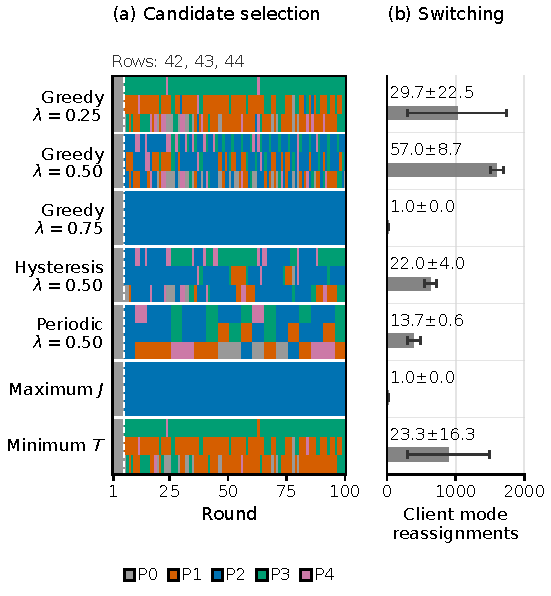
\includegraphics[width=0.98\columnwidth]{experiment_selection_switching.pdf}
		\caption{Candidate selection and switching behavior across three
			seeds. (a) Executed candidate sequences. Within each strategy,
			rows correspond to seeds 42, 43, and 44 from top to bottom;
			rounds 1 to 5 share the common $P_0$ initialization.
			(b) Gray bars and horizontal error bars show the mean and
			sample standard deviation of total client mode changes.
			Numbers above the bars report candidate changes between
			adjacent rounds as mean $\pm$ sample standard deviation.}
		\label{fig:selection_switching}
	\end{figure}	
	\subsection{Learning Performance and System Tradeoffs}
	\label{sec:exp_tradeoffs}
	\label{sec:exp_accuracy_latency}
	Figure~\ref{fig:greedy_fixed_accuracy_latency} compares the final
	test loss and cumulative recorded system latency of the three Greedy
	weights with all five fixed candidates after 100 rounds. This
	comparison examines how different weights affect the final
	learning--latency tradeoff relative to fixed mode distributions.
	Table~\ref{tab:final_tradeoffs} extends the comparison to all
	15 strategies and includes communication and computation costs.
	
	To assess the benefits of dynamic selection,
	each Greedy strategy is compared with a
	Fixed strategy at a similar final loss level.
	Greedy $\lambda=0.25$ and $\lambda=0.50$
	achieve lower mean cumulative latency than
	Fixed $P_3$ and Fixed $P_4$, respectively.
	Greedy $\lambda=0.75$ closely matches
	Fixed $P_2$ in both final loss and
	cumulative latency.
	
	\begin{figure}[t]
		\centering
		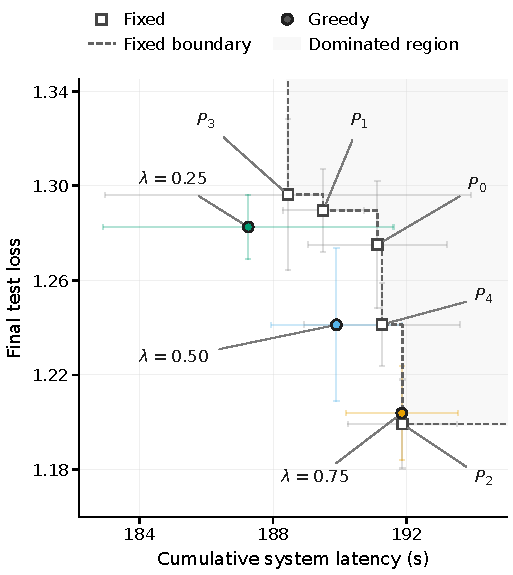
\includegraphics[width=0.96\columnwidth]
		{experiment_final_loss_latency.pdf}
		\caption{Final test loss versus cumulative system
			latency after 100 rounds. The dashed staircase
			marks the observed Fixed frontier, and shading
			indicates the region dominated by Fixed strategies.}		
		\label{fig:greedy_fixed_accuracy_latency}
	\end{figure}
	All three Greedy mean outcomes lie outside the region dominated 
	by the observed Fixed means. Greedy $\lambda=0.25$ achieves a lower
	mean cumulative latency than every Fixed strategy. As $\lambda$
	increases from 0.25 to 0.75, the observed mean final loss decreases
	while mean cumulative latency increases, with $\lambda=0.75$
	approaching Fixed $P_2$. These outcomes associate a stronger
	preference for historical deviation contribution with lower final
	loss at a higher latency cost in this experiment.	
	\begin{table*}[t]
		\centering
		\caption{Learning performance and accumulated system costs for
				all 15 strategies over 100 rounds. Loss is evaluated at round
				100, and accuracy is averaged over rounds 91--100 within each
				seed. Entries are means $\pm$ sample standard deviations
				across three seeds.}
		\label{tab:final_tradeoffs}
		\scriptsize
		\setlength{\tabcolsep}{2.2pt}
		\begin{tabular}{lrrrrrr}
			\toprule
			\textbf{Strategy} & \textbf{Final loss} & \textbf{Accuracy (\%)} &
			\textbf{Cumulative $T$ (s)} & \textbf{Communication (MB)} &
			\textbf{Local steps} & \textbf{Mode changes} \\
			\midrule
			Fixed $P_0$ & $1.2751\pm0.0268$ & $53.24\pm0.97$ & $191.122\pm2.069$ & $10{,}614.5\pm0.0$ & $32{,}000\pm0$ & $0\pm0$ \\
			Fixed $P_1$ & $1.2896\pm0.0175$ & $54.81\pm1.66$ & $189.498\pm1.214$ & $10{,}984.8\pm0.0$ & $30{,}000\pm0$ & $0\pm0$ \\
			Fixed $P_2$ & $1.1992\pm0.0188$ & $54.97\pm0.78$ & $191.868\pm1.628$ & $12{,}836.0\pm0.0$ & $40{,}000\pm0$ & $0\pm0$ \\
			Fixed $P_3$ & $1.2962\pm0.0320$ & $53.47\pm0.84$ & $188.447\pm5.468$ & $9{,}750.5\pm0.0$ & $30{,}000\pm0$ & $0\pm0$ \\
			Fixed $P_4$ & $1.2413\pm0.0174$ & $54.44\pm0.17$ & $191.253\pm2.324$ & $12{,}342.4\pm0.0$ & $36{,}000\pm0$ & $0\pm0$ \\
			\midrule
			Greedy $\lambda=0.25$ & $1.2826\pm0.0136$ & $53.57\pm0.85$ & $187.258\pm4.344$ & $10{,}506.7\pm577.6$ & $30{,}693\pm566$ & $1{,}021.7\pm715.9$ \\
			Greedy $\lambda=0.50$ & $1.2412\pm0.0323$ & $54.29\pm1.19$ & $189.896\pm1.948$ & $11{,}782.8\pm275.0$ & $35{,}600\pm1{,}393$ & $1{,}601.3\pm96.6$ \\
			Greedy $\lambda=0.75$ & $1.2038\pm0.0200$ & $54.95\pm0.85$ & $191.851\pm1.668$ & $12{,}724.9\pm0.0$ & $39{,}600\pm0$ & $20.0\pm0.0$ \\
			Hysteresis $\lambda=0.50$ & $1.2329\pm0.0313$ & $54.64\pm0.45$ & $189.909\pm3.518$ & $11{,}850.3\pm522.1$ & $36{,}213\pm1{,}633$ & $634.0\pm83.5$ \\
			Periodic $\lambda=0.50$ & $1.2526\pm0.0390$ & $53.40\pm1.67$ & $190.154\pm2.549$ & $11{,}591.5\pm154.4$ & $34{,}833\pm1{,}518$ & $394.3\pm88.2$ \\
			Maximum $J$ & $1.2038\pm0.0200$ & $54.95\pm0.85$ & $191.851\pm1.668$ & $12{,}724.9\pm0.0$ & $39{,}600\pm0$ & $20.0\pm0.0$ \\
			Minimum $T$ & $1.2880\pm0.0192$ & $53.28\pm1.03$ & $187.245\pm4.337$ & $10{,}421.9\pm510.9$ & $30{,}307\pm189$ & $895.0\pm597.6$ \\
			\midrule
			Pure $FL_E$ & $1.4146\pm0.0224$ & $52.31\pm1.44$ & $73.117\pm0.254$ & $10{,}121.1\pm0.0$ & $20{,}000\pm0$ & $0\pm0$ \\
			Pure $FL_{EC}$ & $1.1047\pm0.0103$ & $56.65\pm0.68$ & $185.558\pm0.736$ & $17{,}525.8\pm0.0$ & $60{,}000\pm0$ & $0\pm0$ \\
			Pure $FL_C$ & $1.4146\pm0.0224$ & $52.31\pm1.44$ & $83.733\pm0.358$ & $4{,}937.1\pm0.0$ & $20{,}000\pm0$ & $0\pm0$ \\
			\bottomrule
		\end{tabular}
	\end{table*}
	
	Pure $FL_{EC}$ achieves the lowest mean final loss,
	$1.1047\pm0.0103$, and the highest mean accuracy over rounds
	91--100, $56.65\pm0.68\%$, while executing $60{,}000\pm0$
	local steps and transmitting $17{,}525.8\pm0.0$ MB.
	At the other extreme, pure $FL_E$ has the shortest mean recorded
	latency, and pure $FL_C$ transmits the least data, but both finish at a
	mean loss of 1.4146.
	
	Across the means of the 15 observed strategies,
	local steps and final test loss have Pearson
	correlation $-0.961$, whereas local steps
	and mean test accuracy over the last 10 rounds
	have correlation $0.915$.
	More local work therefore coincides with
	lower loss and higher accuracy in this matrix.
	The strong association highlights training
	workload as an important factor when comparing
	collaboration strategies. Complementarily,
	Fig.~\ref{fig:round6_candidate_jt} shows that
	the initial $J$ ranking of $P_2$, $P_0$, and
	$P_3$ agrees with their subsequent loss
	reductions over five rounds.
	
	All 45 strategy runs contain 100 rounds, reach Cloud version 100,
	record 100 acknowledgements and zero pending units, and remain within
	$\epsilon=8$. Across the dynamic strategies, the mean per round Python
	selection time ranges from 7.34 to 7.68 ms; it is recorded separately
	and is not included in simulated system latency.
	\begin{figure*}[t]
		\centering
		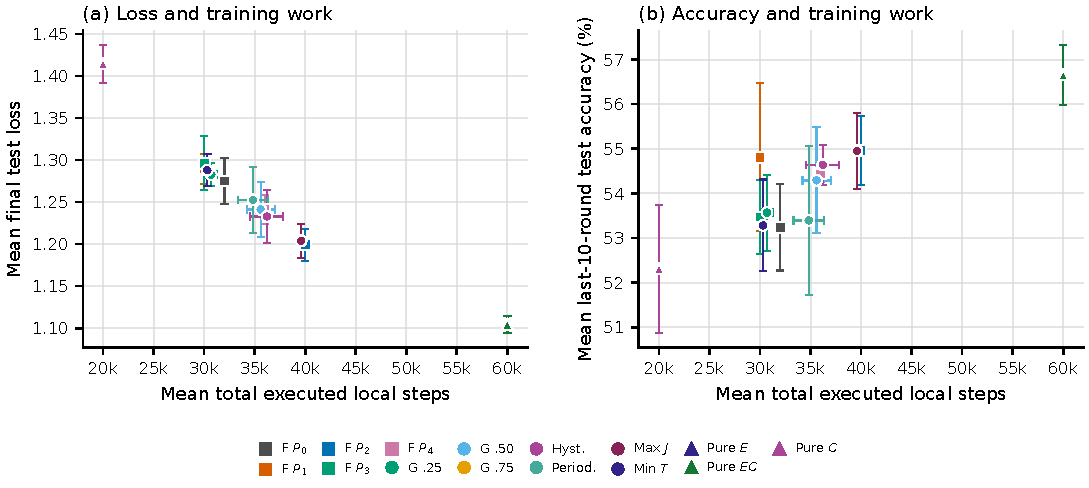
\includegraphics[width=0.98\textwidth]{experiment_final_performance_vs_local_steps.pdf}
		\caption{Final learning performance and total executed local steps for
			the 15 strategies over three seeds. Points and bidirectional error bars
			show the mean and sample standard deviation. Panel (a) relates local
			steps to final test loss, and panel (b) relates local steps to final
			test accuracy.}
		\label{fig:learning_work_relationships}
	\end{figure*}
	
	\subsection{Discussion and Limitations}
	\label{sec:experiment_limits}
	
	
	The historical aggregate update deviation score
	summarizes how the weighted historical deviation
	estimates affect the predicted Cloud update
	relative to the global reference.
	The proposed score does not explicitly model
	the effect of differential privacy noise.
	Instead, it is constructed from historical
	updates generated under differential privacy,
	allowing the effects of privacy protection
	on update characteristics to be indirectly
	reflected in the evaluation of candidate
	mode distributions.
	This avoids the need to separately estimate
	the impact of privacy noise on learning
	performance during candidate evaluation.
	
	Within the finite candidate set, a larger weight on $J$ moves the selector from seed dependent low latency choices toward the larger historical deviation contribution of $P_2$. The resulting high weight strategy attains a competitive loss among the mixed candidates. This supports the limited conclusion that the joint utility produces an observable learning and system cost tradeoff under its declared preferences. It does not establish that larger $J$ causes lower loss, predicts accuracy, or separately identifies the effect of privacy noise.
	
	Several limitations bound this evidence. The reported matrix uses only three seeds, Fashion MNIST, LeNet 5, one topology, and one range of modeled heterogeneity. CIFAR 10, ResNet 18, larger model payloads, and broader topologies require separate validation. The five candidates cover only a small subset of possible client distributions. The network model does not include shared link contention or a physical deployment. Larger models may increase communication,
	local computation, aggregation, and evaluation of the parameter vectors used by $J$, but this scaling effect is not tested here. Finally, candidate scoring and execution use the same implementation timeline, so the online comparisons are internally consistent. 
	\FloatBarrier
	
	\section{Conclusion}
	\label{sec:conclusion}
	This paper presented a dynamic collaboration reconfiguration framework for hierarchical federated learning under resource and lifetime privacy constraints. The framework adapts execution paths and aggregation strategies to the current system state.
	
	Candidate mode distributions are evaluated using
	historical update deviation contributions and system
	latency. The two criteria are normalized and combined
	into a joint utility. At each decision point, Greedy
	selection chooses the feasible candidate with the
	highest current joint utility under resource and
	lifetime privacy constraints. Hysteresis and Periodic
	selection impose additional switching rules and may
	retain the current candidate instead of switching
	to the candidate with the highest current utility.
	Future work will evaluate the framework using more diverse datasets and model architectures. These evaluations will examine whether historical update deviation contributions remain effective for guiding candidate selection under different learning and system conditions. The computational overhead of candidate selection will also be assessed. Further validation will combine online profiling with physical deployment across the Cloud, Edges, and clients.
	
	\appendix
	\bibliographystyle{elsarticle-num}
	\bibliography{refs}
	
\end{document}
